\documentclass[11pt, a4paper, logo, copyright, nonumbering]{deepseek}
\usepackage[authoryear, sort&compress, round]{natbib}
\usepackage{dblfloatfix}
\usepackage{ulem}
\usepackage{caption}
\usepackage{dramatist}
\usepackage{xspace}
\usepackage{pifont} %
\usepackage{multirow}
\usepackage{tcolorbox}
\usepackage{xltabular}
\usepackage{longtable}
\usepackage{hyperref}
\interfootnotelinepenalty=10000

\usepackage{amsfonts}
\usepackage{amsmath}
\usepackage{amssymb}
\usepackage{lineno}
\usepackage{multirow}
\usepackage{adjustbox}

\usepackage[bottom]{footmisc}

\usepackage{CJKutf8}
\usepackage{subfigure}
\usepackage{setspace}

\usepackage{dsfont}
\usepackage{array} %
\usepackage{tabularx} %
\usepackage{subfigure} %
\usepackage{xcolor} %
\usepackage{tabularx}
\usepackage{booktabs}

\usepackage{lipsum}  %
\usepackage{multicol} %




\makeatletter
\def\@BTrule[#1]{%
  \ifx\longtable\undefined
    \let\@BTswitch\@BTnormal
  \else\ifx\hline\LT@hline
    \nobreak
    \let\@BTswitch\@BLTrule
  \else
     \let\@BTswitch\@BTnormal
  \fi\fi
  \global\@thisrulewidth=#1\relax
  \ifnum\@thisruleclass=\tw@\vskip\@aboverulesep\else
  \ifnum\@lastruleclass=\z@\vskip\@aboverulesep\else
  \ifnum\@lastruleclass=\@ne\vskip\doublerulesep\fi\fi\fi
  \@BTswitch}
\makeatother

\addto\extrasenglish{
    \def\chapterautorefname{Chapter}%
    \def\sectionautorefname{Section}%
    \def\paragraphautorefname{Section}
    \def\subparagraphautorefname{Section}
    \def\paragraphautorefname{Paragraph}%
    \def\tableautorefname{Table}%
    \def\equationautorefname{Equation}%
}

\newenvironment{indentchunk}[1]%
 {\begin{list}{}%
         {\setlength{\leftmargin}{#1}}%
         \item[]%
 }
 {\end{list}}
 
\bibliographystyle{abbrvnat}

\reportnumber{001} %

\renewcommand{\today}{}

\title{\centering DeepSeek-R1: Incentivizing Reasoning Capability in LLMs via Reinforcement Learning}


\author[*]{
DeepSeek-AI
\\
\small
\texttt{research@deepseek.com}
}
\newcommand{\lstm}{\textsc{LSTM}}
\newcommand{\ffw} {\textsc{Ffw}}
\newcommand{\attn}{\textsc{Attn}}
\newcommand{\encoder} {\textsc{Encoder}}
\newcommand{\key} {\textsc{Key}}
\newcommand{\query} {\textsc{Query}}
\newcommand{\ccca}{\textsc{Cca}}
\newcommand{\crossattention}{\textsc{Ca}}
\newcommand{\softmax}{\textrm{softmax}}
\newcommand{\ret}{\textsc{Ret}}
\newcommand{\block}{\textsc{Block}}
\newcommand{\MassiveText} {Massive Text}
\newcommand{\bert}{\textsc{Bert}\xspace}
\newcommand{\model}{\textsc{Model}}
\renewcommand{\encoder}{\textsc{Encoder}}
\newcommand{\knnlm}{k\textrm{NN-LM}}
\newcommand{\knn}{k\textrm{NN}}
\newcommand{\spalm}{\textsc{Spalm}}
\newcommand{\dpr}{\textsc{Dpr}}
\newcommand{\rag}{\textsc{RAG}}
\newcommand{\realm}{\textsc{Realm}}
\newcommand{\fid}{\textsc{FiD}}
\newcommand{\emdr}{\textsc{Emdr}^2}
\newcommand{\retro}{\textsc{Retro}\xspace}
\newcommand{\retroon}{\textsc{Retro[On]}\xspace}
\newcommand{\retrooff}{\textsc{Retro[Off]}\xspace}
\newcommand{\retrofit}{\textsc{Retro}fit\xspace}
\newcommand{\retrofitting}{\textsc{Retro}fitting\xspace}
\newcommand{\lm}{\textsc{Lm}}
\newcommand{\lmc}{\textsc{Lmc}}
\newcommand{\emb}{\textsc{Emb}}
\newcommand{\readout}{\textsc{Read}}
\newcommand{\spli}{\textsc{Split}}
\newcommand{\bpb}{\textrm{bpb}}
\newcommand{\dmodel}{d}
\newcommand{\dffw}{d_{\textrm{ffw}}}
\newcommand{\lcp}{\textrm{LCP}}

\newcommand{\datavisheader}[0]{
$C_u$ colored by loss difference & $C_u$ colored by LCP with $\ret(C_u{-1})$  & $[N_u^1, F_u^1]$ colored by LCP with $C_{u+1}$ & $[N_u^2, F_u^2]$ colored by LCP with $C_{u+1}$\\
$L_{\textsc{\retrooff}} - L_{\retro}\colorbox{cm_0!40}{$ \leq -0.5$}, \colorbox{cm_31!40}{$=0 $},\colorbox{cm_63!40}{$ \geq 0.5$}$
& $ \lcp = $ \colorbox{cm_0!40}{$0$}, \colorbox{cm_12!40}{$1 $}, \colorbox{cm_25!40}{$2 $}, \colorbox{cm_38!40}{$3 $},\colorbox{cm_51!40}{$4 $},\colorbox{cm_63!40}{$ \geq 5 $} & $ \lcp = $  \colorbox{cm_0!40}{$0$}, \colorbox{cm_12!40}{$1 $}, \colorbox{cm_25!40}{$2 $}, \colorbox{cm_38!40}{$3 $},\colorbox{cm_51!40}{$4 $},\colorbox{cm_63!40}{$ \geq 5 $} &
$ \lcp = $ \colorbox{cm_0!40}{$0$}, \colorbox{cm_12!40}{$1 $}, \colorbox{cm_25!40}{$2 $}, \colorbox{cm_38!40}{$3 $},\colorbox{cm_51!40}{$4 $},\colorbox{cm_63!40}{$ \geq 5 $} \\
\toprule}

\newcommand{\samplevisheader}[0]{
Prompt and sample of $\retrooff$  & Prompt and sample of $\retroon$ & $[N_u^1, F_u^1]$ colored by LCP with $C_{u+1}$ & $[N_u^2, F_u^2]$ colored by LCP with $C_{u+1}$\\

&
colored by LCP with $\ret(C_u{-1})$
& & \\

&$ \lcp = $ \colorbox{cm_0!40}{$0$}, \colorbox{cm_12!40}{$1 $}, \colorbox{cm_25!40}{$2 $}, \colorbox{cm_38!40}{$3 $},\colorbox{cm_51!40}{$4 $},\colorbox{cm_63!40}{$ \geq 5 $} & $ \lcp = $  \colorbox{cm_0!40}{$0$}, \colorbox{cm_12!40}{$1 $}, \colorbox{cm_25!40}{$2 $}, \colorbox{cm_38!40}{$3 $},\colorbox{cm_51!40}{$4 $},\colorbox{cm_63!40}{$ \geq 5 $}  &$ \lcp = $ \colorbox{cm_0!40}{$0$}, \colorbox{cm_12!40}{$1 $}, \colorbox{cm_25!40}{$2 $}, \colorbox{cm_38!40}{$3 $},\colorbox{cm_51!40}{$4 $},\colorbox{cm_63!40}{$ \geq 5 $} \\

\toprule}

\newcommand{\NN}{\mathbb{N}}
\newcommand{\CC}{\mathbb{C}}
\newcommand{\GG}{\mathbb{G}}
\newcommand{\LL}{\mathbb{L}}
\newcommand{\PP}{\mathbb{P}}
\renewcommand{\SS}{\mathbb{S}}
\newcommand{\QQ}{\mathbb{Q}}
\newcommand{\RR}{\mathbb{R}}
\newcommand{\VV}{\mathbb{V}}
\newcommand{\ZZ}{\mathbb{Z}}
\newcommand{\FF}{\mathbb{F}}
\newcommand{\KK}{\mathbb{K}}
\newcommand{\TT}{\mathbb{T}}
\newcommand{\UU}{\mathbb{U}}
\newcommand{\EE}{\mathbb{E}}
\newcommand{\XX}{\mathbb{X}}
\newcommand{\YY}{\mathbb{Y}}
\newcommand{\Aa}{\mathcal{A}}
\newcommand{\Bb}{\mathcal{B}}
\newcommand{\Cc}{\mathcal{C}}
\newcommand{\Dd}{\mathcal{D}}
\newcommand{\Ee}{\mathcal{E}}
\newcommand{\Ff}{\mathcal{F}}
\newcommand{\Gg}{\mathcal{G}}
\newcommand{\Hh}{\mathcal{H}}
\newcommand{\Ii}{\mathcal{I}}
\newcommand{\Jj}{\mathcal{J}}
\newcommand{\Kk}{\mathcal{K}}
\newcommand{\Ll}{\mathcal{L}}
\newcommand{\Mm}{\mathcal{M}}
\newcommand{\Nn}{\mathcal{N}}
\newcommand{\Oo}{\mathcal{O}}
\newcommand{\Pp}{\mathcal{P}}
\newcommand{\Qq}{\mathcal{Q}}
\newcommand{\Rr}{\mathcal{R}}
\newcommand{\Ss}{\mathcal{S}}
\newcommand{\Tt}{\mathcal{T}}
\newcommand{\Uu}{\mathcal{U}}
\newcommand{\Vv}{\mathcal{V}}
\newcommand{\Ww}{\mathcal{W}}
\newcommand{\Xx}{\mathcal{X}}
\newcommand{\Yy}{\mathcal{Y}}
\newcommand{\Zz}{\mathcal{Z}}

\newcommand{\al}{\alpha}
\newcommand{\la}{\lambda}
\newcommand{\ga}{\gamma}
\newcommand{\Ga}{\Gamma}
\newcommand{\La}{\Lambda}
\newcommand{\si}{\sigma}
\newcommand{\be}{\beta}
\newcommand{\de}{\delta}
\newcommand{\De}{\Delta}
\renewcommand{\phi}{\varphi}
\renewcommand{\th}{\theta}
\newcommand{\om}{\omega}
\newcommand{\Om}{\Omega}

\newcommand{\hf}{\hat f}
\newcommand{\wtf}{\tilde f}
\newcommand{\tx}{\tilde x}
\newcommand{\ta}{\tilde a}
\newcommand{\tb}{\tilde b}
\newcommand{\ty}{\tilde y}
\newcommand{\tu}{\tilde u}
\newcommand{\tv}{\tilde v}
\newcommand{\tga}{\tilde \ga}
\newcommand{\tf}{\wt{f}}

\newcommand{\ins}[1]{\mathrm{#1}}
\let\Re\relax

\DeclareMathOperator{\Re}{\Rr e}
\DeclareMathOperator{\Imag}{\Ii m}
\DeclareMathOperator{\Ker}{Ker}
\DeclareMathOperator{\Hom}{Hom}
\DeclareMathOperator{\End}{End}
\DeclareMathOperator{\tr}{tr}
\DeclareMathOperator{\Tr}{Tr}
\DeclareMathOperator{\Supp}{Supp}
\DeclareMathOperator{\Sign}{Sign}
\let\Im\relax
\DeclareMathOperator{\Im}{Im}
\DeclareMathOperator{\Corr}{Corr}
\DeclareMathOperator{\sign}{sign}
\DeclareMathOperator{\supp}{supp}

\DeclareMathOperator{\cas}{cas}
\DeclareMathOperator{\sinc}{sinc}
\DeclareMathOperator{\cotan}{cotan}
\DeclareMathOperator{\Card}{Card}
\DeclareMathOperator{\GCD}{GCD}
\DeclareMathOperator{\grad}{grad}
\DeclareMathOperator{\Diag}{Diag}
\DeclareMathOperator{\rank}{rank}
\DeclareMathOperator{\conv}{conv}
\DeclareMathOperator{\interop}{int}

\newcommand{\ps}[2]{\langle #1,#2\rangle}

\newcommand{\Calpha}{\mathrm{C}^\al}
\newcommand{\Cbeta}{\mathrm{C}^\be}
\newcommand{\Cal}{\text{C}^\al}
\newcommand{\Ctwo}{\text{C}^{2}}
\newcommand{\Calt}[1]{\text{C}^{#1}}
\newcommand{\Cder}[1]{\mathscr{C}^{#1}}
\newcommand{\lone}{\ell^1}
\newcommand{\ltwo}{\ell^2}
\newcommand{\linf}{\ell^\infty}
\newcommand{\Lone}{\text{\upshape L}^1}
\newcommand{\Ltwo}{\text{\upshape L}^2}
\newcommand{\Linf}{\text{\upshape L}^\infty}
\newcommand{\lzero}{\ell^0}
\newcommand{\lp}{\ell^p}
\newcommand{\Sun}{\text{S}^1}
\newcommand{\foralls}{\forall \,}
\newcommand{\dd}{\ins{d}}
\renewcommand{\leq}{\leqslant}
\renewcommand{\geq}{\geqslant}

\newcommand{\ol}[1]{\overline{#1}}
\newcommand{\wh}[1]{\widehat{#1}}
\newcommand{\whwh}[1]{\hat{\hat{#1}}}
\newcommand{\wt}[1]{\widetilde{#1}}
\newcommand{\pd}[2]{ \frac{ \partial #1}{\partial #2} }
\newcommand{\pdd}[2]{ \frac{ \partial^2 #1}{\partial #2^2} }
\renewcommand{\epsilon}{\varepsilon}
\renewcommand{\imath}{\mathrm{i}}
\newcommand{\interior}[1]{\ensuremath{\overset{\circ}{#1}}}

\newcommand{\legsymb}[2]{ \genfrac{(}{)}{}{}{#1}{#2} }
\newcommand{\ordin}[2]{ ${#1}^{ \text{#2} }$ }
\newcommand{\dotp}[2]{\langle #1,\,#2\rangle}
\newcommand{\dotps}[2]{\langle #1,\,#2\rangle}
\newcommand{\crossp}[2]{ #1 \hat #2 }
\newcommand{\seg}[2]{\llbracket #1,\,#2 \rrbracket}
\newcommand{\brac}[1]{\left[#1\right]}
\newcommand{\norm}[1]{\left\| #1 \right\|}
\newcommand{\snorm}[1]{\| #1 \|}
\newcommand{\normb}[1]{\Big|\!\Big| #1 \Big |\!\Big|}
\newcommand{\normB}[1]{\left|\!\left| #1 \right|\!\right|}
\DeclareMathOperator{\diverg}{div}
\DeclareMathOperator{\Prox}{Prox}
\newcommand{\normT}[1]{\norm{#1}_{\text{T}}}
\newcommand{\normu}[1]{\norm{#1}_{1}}
\newcommand{\normi}[1]{\norm{#1}_{\infty}}
\newcommand{\normd}[1]{\norm{#1}_{2}}
\newcommand{\normz}[1]{\norm{#1}_{0}}
\newcommand{\abs}[1]{\left\lvert#1\right\rvert}
\newcommand{\absb}[1]{\Big| #1 \Big|}

\newcommand{\func}[4]{ {\left\{  \begin{array}{ccc} #1 & \longrightarrow & #2 \\ #3 & \longmapsto & #4 \end{array}  \right.} }
\newcommand{\Id}{\ins{Id}}
\newcommand{\eqdef}{\triangleq}

\DeclareMathOperator*{\argmin}{argmin}
\DeclareMathOperator*{\argmax}{argmax}

\newcommand{\pa}[1]{\left( #1 \right)}
\newcommand{\bpa}[1]{\big( #1 \big)}
\newcommand{\choice}[1]{
	\left\{
		\begin{array}{l} #1 \end{array}
	\right. }
\newcommand{\set}[1]{ \{ #1 \} }
\newcommand{\condset}[2]{ \left\{ #1 \;;\; #2 \right\} }

\newcommand{\qandq}{ \quad \text{and} \quad }
\newcommand{\qqandqq}{ \qquad \text{and} \qquad }
\newcommand{\qifq}{ \quad \text{if} \quad }
\newcommand{\qqifqq}{ \qquad \text{if} \qquad }
\newcommand{\qwhereq}{ \quad \text{where} \quad }
\newcommand{\qqwhereqq}{ \qquad \text{where} \qquad }
\newcommand{\qwithq}{ \quad \text{with} \quad }
\newcommand{\qqwithqq}{ \qquad \text{with} \qquad }
\newcommand{\qforq}{ \quad \text{for} \quad }
\newcommand{\qqforqq}{ \qquad \text{for} \qquad }
\newcommand{\qqsinceqq}{ \qquad \text{since} \qquad }
\newcommand{\qsinceq}{ \quad \text{since} \quad }
\newcommand{\qarrq}{\quad\Longrightarrow\quad}
\newcommand{\qqarrqq}{\quad\Longrightarrow\quad}
\newcommand{\qiffq}{\quad\Longleftrightarrow\quad}
\newcommand{\qqiffqq}{\qquad\Longleftrightarrow\qquad}
\newcommand{\qsubjq}{ \quad \text{subject to} \quad }
\newcommand{\qqsubjqq}{ \qquad \text{subject to} \qquad }
\newcommand{\qobjq}[1]{\quad \text{#1} \quad}
\newcommand{\qqobjqq}[1]{\quad \text{#1} \quad}

\newlength{\restsubwidth}
\newlength{\restsubheight}
\newlength{\restsubmoreheight}
\setlength{\restsubmoreheight}{4pt}
\newcommand{\rest}[2]{
        \settowidth{\restsubwidth}{\ensuremath{#2}}
        \settoheight{\restsubheight}{\ensuremath{{}_{#2}}}
        \ensuremath{{#1\hskip 0.5pt}_{\vrule\kern2pt\parbox[b][
        4pt][b]{\the\restsubwidth}{
                        \ensuremath{{}_{#2}}}}}
        }



\newcommand{\fix}{\marginpar{FIX}}
\newcommand{\new}{\marginpar{NEW}}
\newcommand{\dsri}{DeepSeek-R1}
\newcommand{\dsro}{DeepSeek-R1-Zero}
\newcommand{\todo}[1]{\textcolor[rgb]{0.8,0,0.2}{#1}}

\begin{abstract}


We introduce our first-generation reasoning models, \dsro{} and \dsri{}. 
\dsro{}, a model trained via large-scale reinforcement learning (RL) without supervised fine-tuning (SFT) as a preliminary step, demonstrates remarkable reasoning capabilities.
Through RL, \dsro{} naturally emerges with numerous powerful and intriguing reasoning behaviors.
However, it encounters challenges such as poor readability, and language mixing. To address these issues and further enhance reasoning performance,
we introduce \dsri{}, which incorporates multi-stage training and cold-start data before RL.
\dsri{} achieves performance comparable to OpenAI-o1-1217 on reasoning tasks. 
To support the research community, we open-source \dsro{}, \dsri{}, and six dense models (1.5B, 7B, 8B, 14B, 32B, 70B) distilled from \dsri{} based on Qwen and Llama.

\end{abstract}

\begin{document}

\maketitle
\begin{figure}[h]
\centering
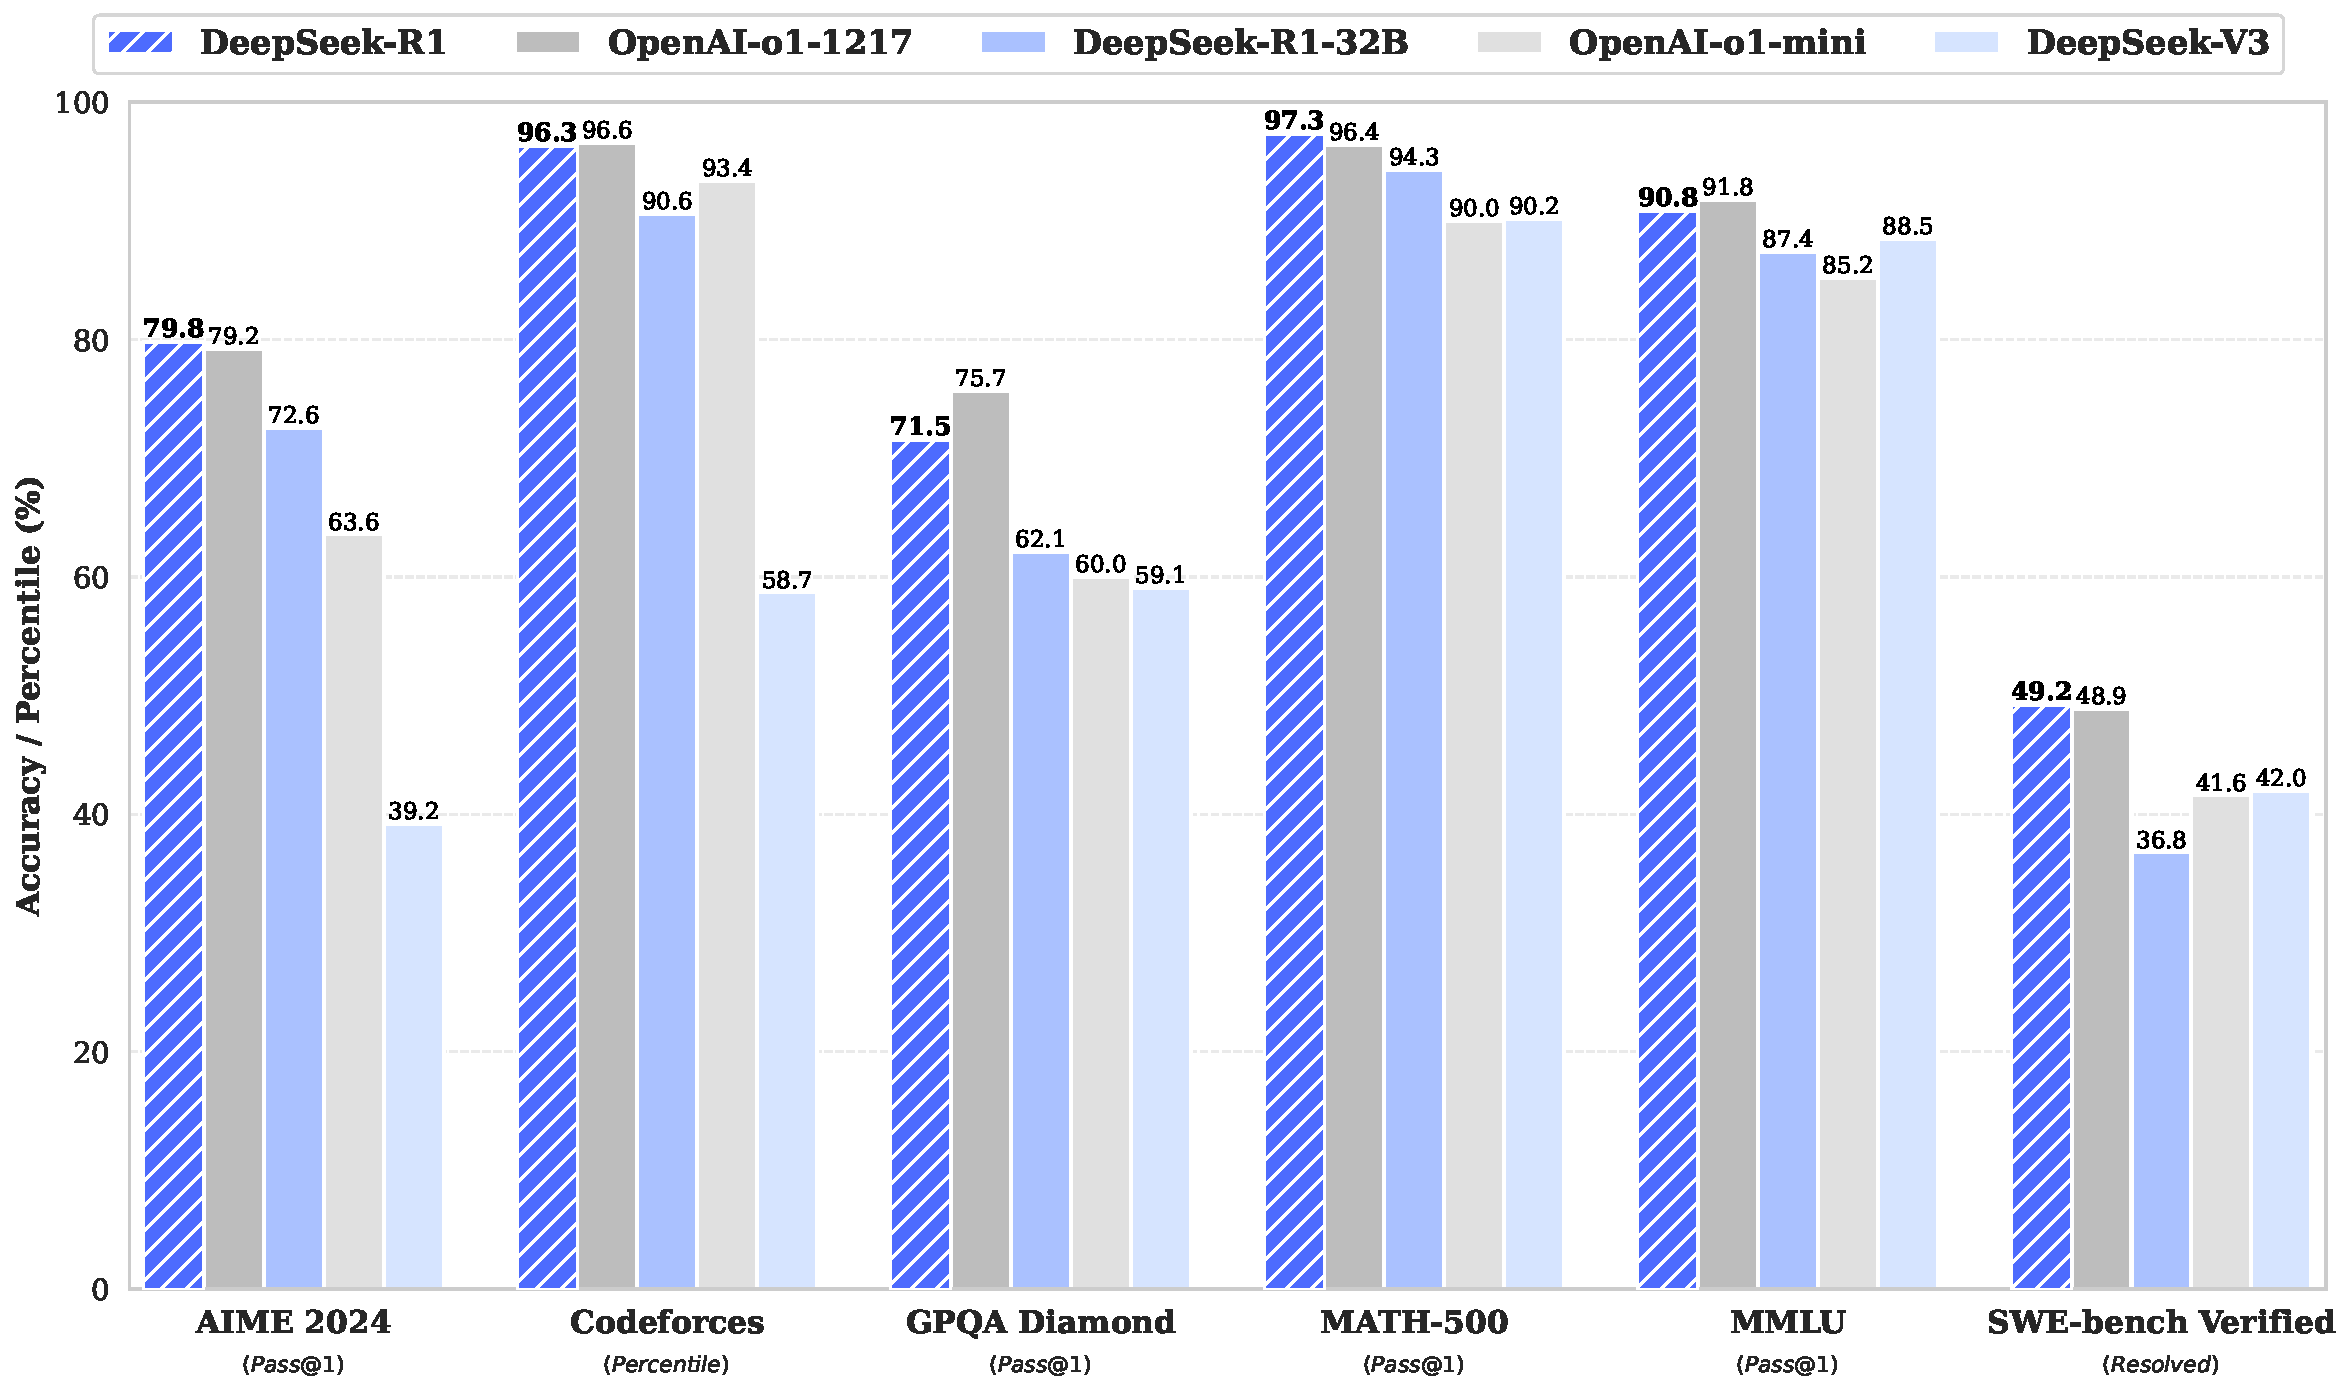
\includegraphics[width=1.0\textwidth]{figures/dsr1_performance.pdf}
\caption{
    \centering
    Benchmark performance of \dsri{}.
}
\label{fig:dsv3_performance}
\end{figure}

\newpage

\begin{spacing}{0.9}
\tableofcontents
\end{spacing}

\newpage

\section{Introduction}
In recent years, Large Language Models~(LLMs) have been undergoing rapid iteration and evolution~\citep{gpt4o,claude35sonnet,gemini1_5}, progressively diminishing the gap towards Artificial General Intelligence~(AGI).

Recently, post-training has emerged as an important component of the full training pipeline. It has been shown to enhance accuracy on reasoning tasks, align with social values, and adapt to user preferences, all while requiring relatively minimal computational resources against pre-training. In the context of reasoning capabilities, OpenAI's o1~\citep{o1} series models were the first to introduce inference-time scaling by increasing the length of the Chain-of-Thought reasoning process. This approach has achieved significant improvements in various reasoning tasks, such as mathematics, coding, and scientific reasoning. However, the challenge of effective test-time scaling remains an open question for the research community. 
Several prior works have explored various approaches, including process-based reward models \citep{uesato2022solving, lightman2023let,mathshepherd}, reinforcement learning \citep{kumar2024training}, and search algorithms such as Monte Carlo Tree Search and Beam Search \citep{feng2024alphazeroliketreesearchguidelarge,xin2024deepseekproverv15harnessingproofassistant,AlphaGeometryTrinh2024}.
However, none of these methods has achieved general reasoning performance comparable to OpenAI's o1 series models.

In this paper, we take the first step toward improving language model reasoning capabilities using pure reinforcement learning (RL).
Our goal is to explore the potential of LLMs to develop reasoning capabilities without any supervised data, focusing on their self-evolution through a pure RL process.
Specifically, we use DeepSeek-V3-Base as the base model and employ GRPO~\citep{deepseekmath} as the RL framework to improve model performance in reasoning.
During training, \dsro{} naturally emerged with numerous powerful and interesting reasoning behaviors. After thousands of RL steps, \dsro{} exhibits super performance on reasoning benchmarks. 
For instance, the pass@1 score on AIME 2024 increases from 15.6\% to 71.0\%, and with majority voting, the score further improves to 86.7\%, matching the performance of OpenAI-o1-0912.


However, \dsro{} encounters challenges such as poor readability, and language mixing. To address these issues and further enhance reasoning performance, we introduce \dsri{}, which incorporates a small amount of cold-start data and a multi-stage training pipeline.
Specifically, we begin by collecting thousands of cold-start data to fine-tune the DeepSeek-V3-Base model. Following this, we perform reasoning-oriented RL like \dsro{}. Upon nearing convergence in the RL process, we create new SFT data through rejection sampling on the RL checkpoint, combined with supervised data from DeepSeek-V3 in domains such as writing, factual QA, and self-cognition, and then retrain the DeepSeek-V3-Base model. After fine-tuning with the new data, the checkpoint undergoes an additional RL process, taking into account prompts from all scenarios. After these steps, we obtained a checkpoint referred to as \dsri{}, which achieves performance on par with OpenAI-o1-1217.

We further explore distillation from \dsri{} to smaller dense models. Using Qwen2.5-32B~\citep{qwen2_5} as the base model, direct distillation from \dsri{} outperforms applying RL on it. This demonstrates that the reasoning patterns discovered by larger base models are crucial for improving reasoning capabilities.  We open-source the distilled Qwen and Llama~\citep{llama3} series. Notably, our distilled 14B model outperforms state-of-the-art open-source QwQ-32B-Preview~\citep{QwQ} by a large margin, and the distilled 32B and 70B models set a new record on the reasoning benchmarks among dense models.


\subsection{Contributions}

\paragraph{Post-Training: Large-Scale Reinforcement Learning on the Base Model}
\begin{itemize}[topsep=0pt]
    \item 
    We directly apply RL to the base model without relying on supervised fine-tuning (SFT) as a preliminary step. This approach allows the model to explore chain-of-thought (CoT) for solving complex problems, resulting in the development of \dsro{}. \dsro{} demonstrates capabilities such as self-verification, reflection, and generating long CoTs, marking a significant milestone for the research community. Notably, it is the first open research to validate that reasoning capabilities of LLMs can be incentivized purely through RL, without the need for SFT. This breakthrough paves the way for future advancements in this area.
    \item
    We introduce our pipeline to develop \dsri{}. The pipeline incorporates two RL stages aimed at discovering improved reasoning patterns and aligning with human preferences, as well as two SFT stages that serve as the seed for the model's reasoning and non-reasoning capabilities.
    We believe the pipeline will benefit the industry by creating better models. 
    
\end{itemize}


\paragraph{Distillation: Smaller Models Can Be Powerful Too}
\begin{itemize}[topsep=0pt]
    \item We demonstrate that the reasoning patterns of larger models can be distilled into smaller models, resulting in better performance compared to the reasoning patterns discovered through RL on small models. The open source \dsri{}, as well as its API, will benefit the research community to distill better smaller models in the future. 
    \item Using the reasoning data generated by \dsri{}, we fine-tuned several dense models that are widely used in the research community. The evaluation results demonstrate that the distilled smaller dense models perform exceptionally well on benchmarks.
    DeepSeek-R1-Distill-Qwen-7B achieves 55.5\% on AIME 2024, surpassing QwQ-32B-Preview. Additionally, DeepSeek-R1-Distill-Qwen-32B scores 72.6\% on AIME 2024, 94.3\% on MATH-500, and 57.2\% on LiveCodeBench. These results significantly outperform previous open-source models and are comparable to o1-mini.
    We open-source distilled 1.5B, 7B, 8B, 14B, 32B, and 70B checkpoints based on Qwen2.5 and Llama3 series to the community.
\end{itemize}

\subsection{Summary of Evaluation Results}
\begin{itemize}[topsep=0pt]
    
    \item \textbf{Reasoning tasks}: 
    (1)
   \dsri{} achieves a score of 79.8\% Pass@1 on AIME 2024, slightly surpassing OpenAI-o1-1217. On MATH-500, it attains an impressive score of 97.3\%, performing on par with OpenAI-o1-1217 and significantly outperforming other models. 
    (2)
    On coding-related tasks, \dsri{} demonstrates expert level in code competition tasks, as it achieves 2,029 Elo rating on Codeforces outperforming 96.3\% human participants in the competition. 
    For engineering-related tasks,  \dsri{} performs slightly better than DeepSeek-V3, which could help developers in real world tasks.
    
    \item \textbf{Knowledge}:
On benchmarks such as MMLU, MMLU-Pro, and GPQA Diamond, \dsri{} achieves outstanding results, significantly outperforming DeepSeek-V3 with scores of 90.8\% on MMLU, 84.0\% on MMLU-Pro, and 71.5\% on GPQA Diamond. While its performance is slightly below that of OpenAI-o1-1217 on these benchmarks, \dsri{} surpasses other closed-source models, demonstrating its competitive edge in educational tasks. On the factual benchmark SimpleQA, \dsri{} outperforms DeepSeek-V3, demonstrating its capability in handling fact-based queries. A similar trend is observed where OpenAI-o1 surpasses 4o on this benchmark.
    \item \textbf{Others}: \dsri{} also excels in a wide range of tasks, including creative writing, general question answering, editing, summarization, and more. It achieves an impressive length-controlled win-rate of 87.6\% on AlpacaEval 2.0 and a win-rate of 92.3\% on ArenaHard, showcasing its strong ability to intelligently handle non-exam-oriented queries. Additionally, \dsri{} demonstrates outstanding performance on tasks requiring long-context understanding, substantially outperforming DeepSeek-V3 on long-context benchmarks.
\end{itemize}


\section{Approach}
\subsection{Overview}
Previous work has heavily relied on large amounts of supervised data to enhance model performance. In this study, we demonstrate that reasoning capabilities can be significantly improved through large-scale reinforcement learning (RL), even without using supervised fine-tuning (SFT) as a cold start. Furthermore, performance can be further enhanced with the inclusion of a small amount of cold-start data. In the following sections, we present: (1) \dsro{}, which applies RL directly to the base model without any SFT data, and (2) \dsri{}, which applies RL starting from a checkpoint fine-tuned with thousands of long Chain-of-Thought (CoT) examples. 3) Distill the reasoning capability from \dsri{} to small dense models. 


\subsection{ \dsro{}: Reinforcement Learning on the Base Model}
\label{sec:ds-zero}
Reinforcement learning has demonstrated significant effectiveness in reasoning tasks, as evidenced by our previous works \citep{mathshepherd,deepseekmath}. 
However, these works heavily depended on supervised data, which are time-intensive to gather.
In this section, we explore the potential of LLMs to develop reasoning capabilities \textbf{without any supervised data}, focusing on their self-evolution through a pure reinforcement learning process. 
We start with a brief overview of our RL algorithm, followed by the presentation of some exciting results, and hope this provides the community with valuable insights.

\subsubsection{Reinforcement Learning Algorithm}
\paragraph{Group Relative Policy Optimization} In order to save the training costs of RL, we adopt Group Relative Policy Optimization~(GRPO) \citep{deepseekmath}, which foregoes the critic model that is typically the same size as the policy model, and estimates the baseline from group scores instead. 
Specifically, for each question $q$, GRPO samples a group of outputs $\{o_1, o_2, \cdots, o_G\}$ from the old policy $\pi_{\theta_{old}}$ and then optimizes the policy model $\pi_{\theta}$ by maximizing the following objective:
\begin{equation}
\begin{split}
    \mathcal{J}_{GRPO}(\theta) &= \mathbb{E}{[q \sim P(Q), \{o_i\}_{i=1}^G \sim \pi_{\theta_{old}}(O|q)]}  \\
    & \frac{1}{G}\sum_{i=1}^G \left( \min \left( \frac{\pi_\theta(o_i |q)}{\pi_{\theta_{old}}(o_i |q)} A_i, \text{clip} \left( \frac{\pi_\theta(o_i |q)}{\pi_{\theta_{old}}(o_i |q)}, 1 - \epsilon, 1 + \epsilon \right)  A_i \right) - \beta \mathbb{D}_{KL}\left(\pi_{\theta} || \pi_{ref}\right)\right) ,
\end{split}
\label{eq:GRPO-obj}
\end{equation}
\begin{equation}
    \mathbb{D}_{KL}\left(\pi_{\theta} || \pi_{ref}\right) = \frac{\pi_{ref}(o_i|q)}{\pi_{\theta}(o_i|q)}- \log\frac{\pi_{ref}(o_i|q)}{\pi_{\theta}(o_i|q)} - 1,
\end{equation}
where $\epsilon$ and $\beta$ are hyper-parameters, and $A_i$ is the advantage, computed using a group of rewards $\{r_1, r_2, \ldots, r_G\}$ corresponding to the outputs within each group:
\begin{equation}
    A_i = \frac{r_i - {\mathrm mean(\{r_1, r_2, \cdots, r_G\})}}{{\mathrm std(\{r_1, r_2, \cdots, r_G\})}}.
\end{equation}


\begin{table}[t]
    \centering
    \small
    \begin{tabular}{l}
    \toprule
    A conversation between User and Assistant. The user asks a question, and the Assistant solves it. \\
     The assistant first thinks about the reasoning process in the mind and then provides the user \\ with the answer.
     The reasoning process and answer are enclosed within <think> </think> and \\<answer> </answer> tags, respectively, i.e., <think> reasoning process here </think> \\ <answer> answer here </answer>. 
     User: \textcolor{red}{prompt}. Assistant: \\
     \bottomrule
    \end{tabular}
    \caption{Template for \dsro{}. \textcolor{red}{prompt} will be replaced with the specific reasoning question during training.}
    \label{tab:r0_template}
\end{table}




\subsubsection{Reward Modeling} The reward is the source of the training signal, which decides the optimization direction of RL.
To train \dsro{}, we adopt a rule-based reward system that mainly consists of two types of rewards: 
\begin{itemize}[topsep=0pt]
    \item \textbf{Accuracy rewards}: The accuracy reward model evaluates whether the response is correct. For example, in the case of math problems with deterministic results, the model is required to provide the final answer in a specified format (e.g., within a box), enabling reliable rule-based verification of correctness. Similarly, for LeetCode problems, a compiler can be used to generate feedback based on predefined test cases.
    \item \textbf{Format rewards}: In addition to the accuracy reward model, we employ a format reward model that enforces the model to put its thinking process between `<think>' and `</think>' tags.
\end{itemize}
We do not apply the outcome or process neural reward model in developing  \dsro{}, because we find that the neural reward model may suffer from reward hacking in the large-scale reinforcement learning process, and retraining the reward model needs additional training resources and it complicates the whole training pipeline.


\subsubsection{Training Template}

To train \dsro{}, we begin by designing a straightforward template that guides the base model to adhere to our specified instructions. As depicted in Table \ref{tab:r0_template}, this template requires \dsro{} to first produce a reasoning process, followed by the final answer. We intentionally limit our constraints to this structural format, avoiding any content-specific biases—such as mandating reflective reasoning or promoting particular problem-solving strategies—to ensure that we can accurately observe the model's natural progression during the RL process.



\subsubsection{Performance, Self-evolution Process and Aha Moment of \dsro{}}

\paragraph{Performance of \dsro{}}

\begin{table}[t]
    \centering
    \resizebox{\linewidth}{!}{
    \begin{tabular}{@{}l *{6}{c} @{}}
    \toprule
    \multirow{3}{*}{\centering\textbf{Model}} & \multicolumn{2}{c}{\multirow{2}{*}{\textbf{AIME 2024}}} & \multirow{2}{*}{\textbf{MATH-500}} & \textbf{GPQA} & \textbf{LiveCode} & \multirow{2}{*}{\textbf{CodeForces}} \\
     &  & &  & \textbf{Diamond} & \textbf{Bench} \\
    \cmidrule(lr){2-3}
     & pass@1 & cons@64 & pass@1 &  pass@1 & pass@1 & rating \\
    \midrule
    \textbf{OpenAI-o1-mini} & 63.6 & 80.0 & 90.0  & 60.0 & 53.8 & 1820 \\
    \textbf{OpenAI-o1-0912} & 74.4  & 83.3  & 94.8  & 77.3 & 63.4 & 1843 \\
    \midrule
    \textbf{\dsro{}} & 71.0 & 86.7 & 95.9 & 73.3 & 50.0 & 1444 \\
    \bottomrule
    \end{tabular}
    }
    \caption{Comparison of \dsro{} and OpenAI o1 models on reasoning-related benchmarks.}
    \label{tab:r1-zero}
\end{table}

\begin{figure}
    \centering
    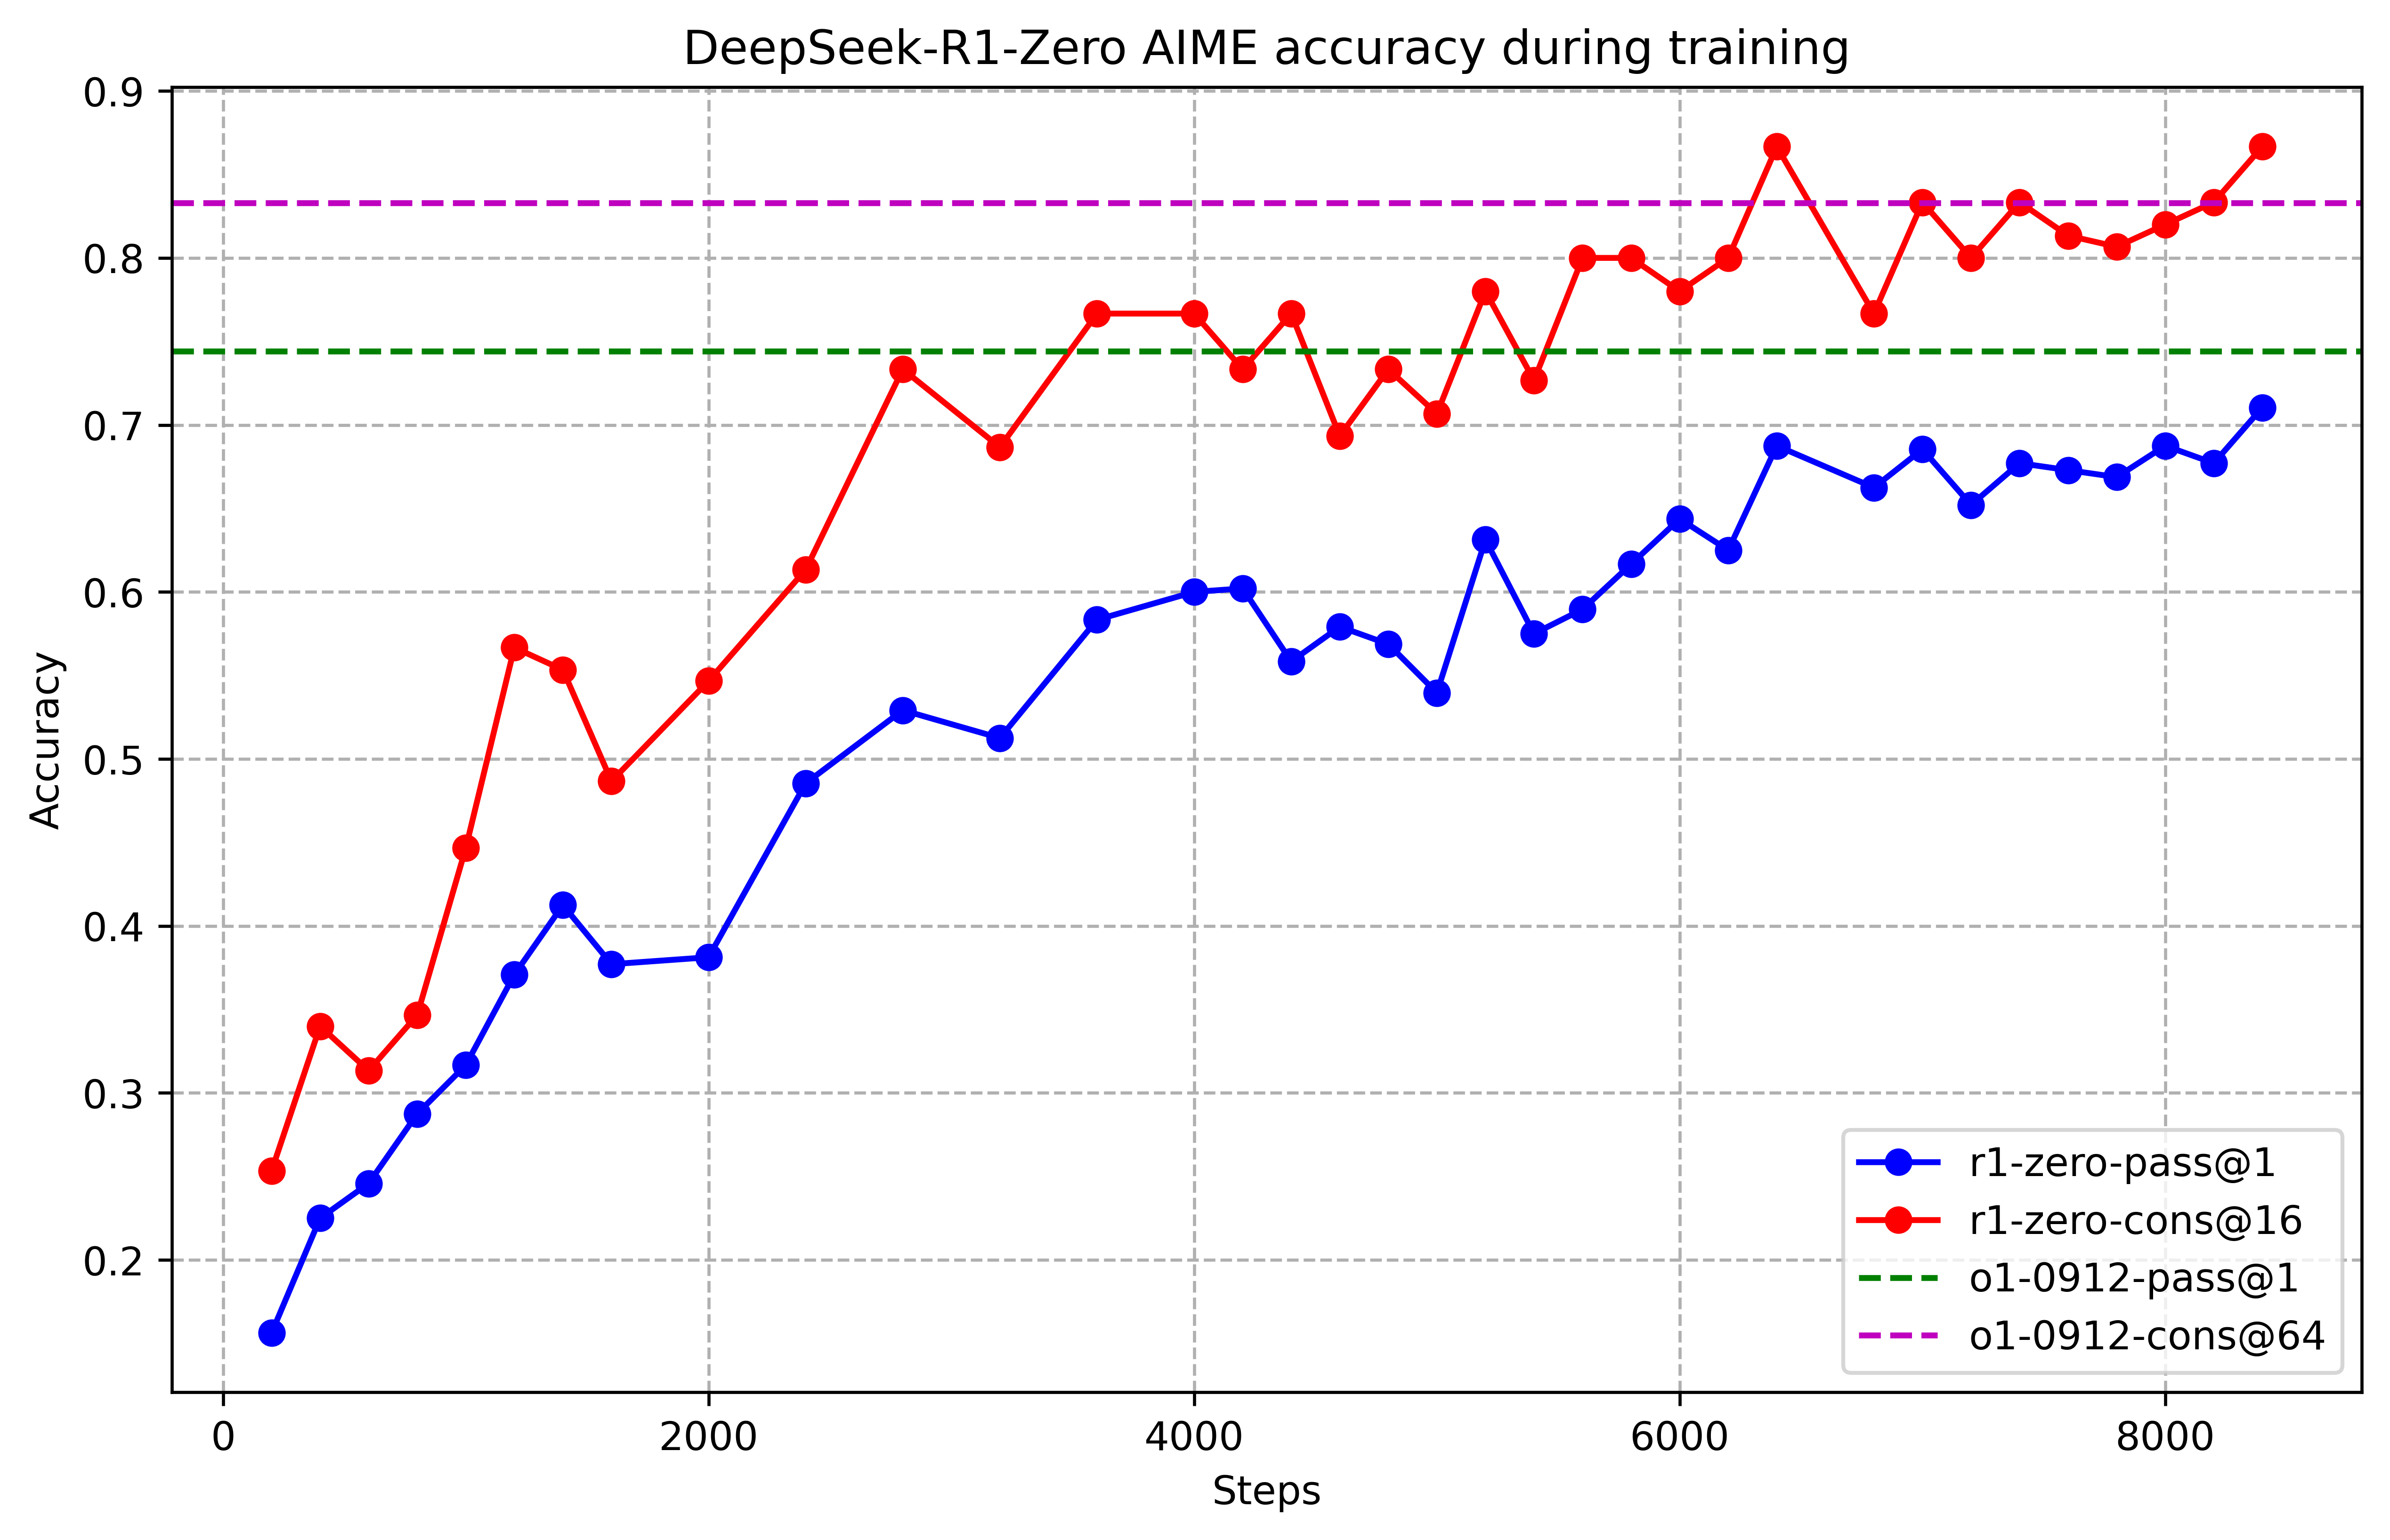
\includegraphics[width=0.75\linewidth]{figures/plot_aime_with_maj.png}
    \caption{AIME accuracy of \dsro{} during training. For each question, we sample 16 responses and calculate the overall average accuracy to ensure a stable evaluation.}
    \label{fig:zero-training-performance}
\end{figure}


Figure \ref{fig:zero-training-performance} depicts the performance trajectory of \dsro{} on the AIME 2024 benchmark throughout the RL training process. As illustrated, \dsro{} demonstrates a steady and consistent enhancement in performance as the RL training advances. Notably, the average pass@1 score on AIME 2024 shows a significant increase, jumping from an initial 15.6\% to an impressive 71.0\%, reaching performance levels comparable to OpenAI-o1-0912. This significant improvement highlights the efficacy of our RL algorithm in optimizing the model's performance over time.

Table \ref{tab:r1-zero} provides a comparative analysis between \dsro{} and OpenAI's o1-0912 models across a variety of reasoning-related benchmarks. The findings reveal that RL empowers \dsro{} to attain robust reasoning capabilities without the need for any supervised fine-tuning data.
This is a noteworthy achievement, as it underscores the model's ability to learn and generalize effectively through RL alone. Additionally, the performance of \dsro{} can be further augmented through the application of majority voting. For example, when majority voting is employed on the AIME benchmark, \dsro{}'s performance escalates from 71.0\% to 86.7\%, thereby exceeding the performance of OpenAI-o1-0912. 
The ability of \dsro{} to achieve such competitive performance, both with and without majority voting, highlights its strong foundational capabilities and its potential for further advancements in reasoning tasks.

\begin{figure}[t]
    \centering
    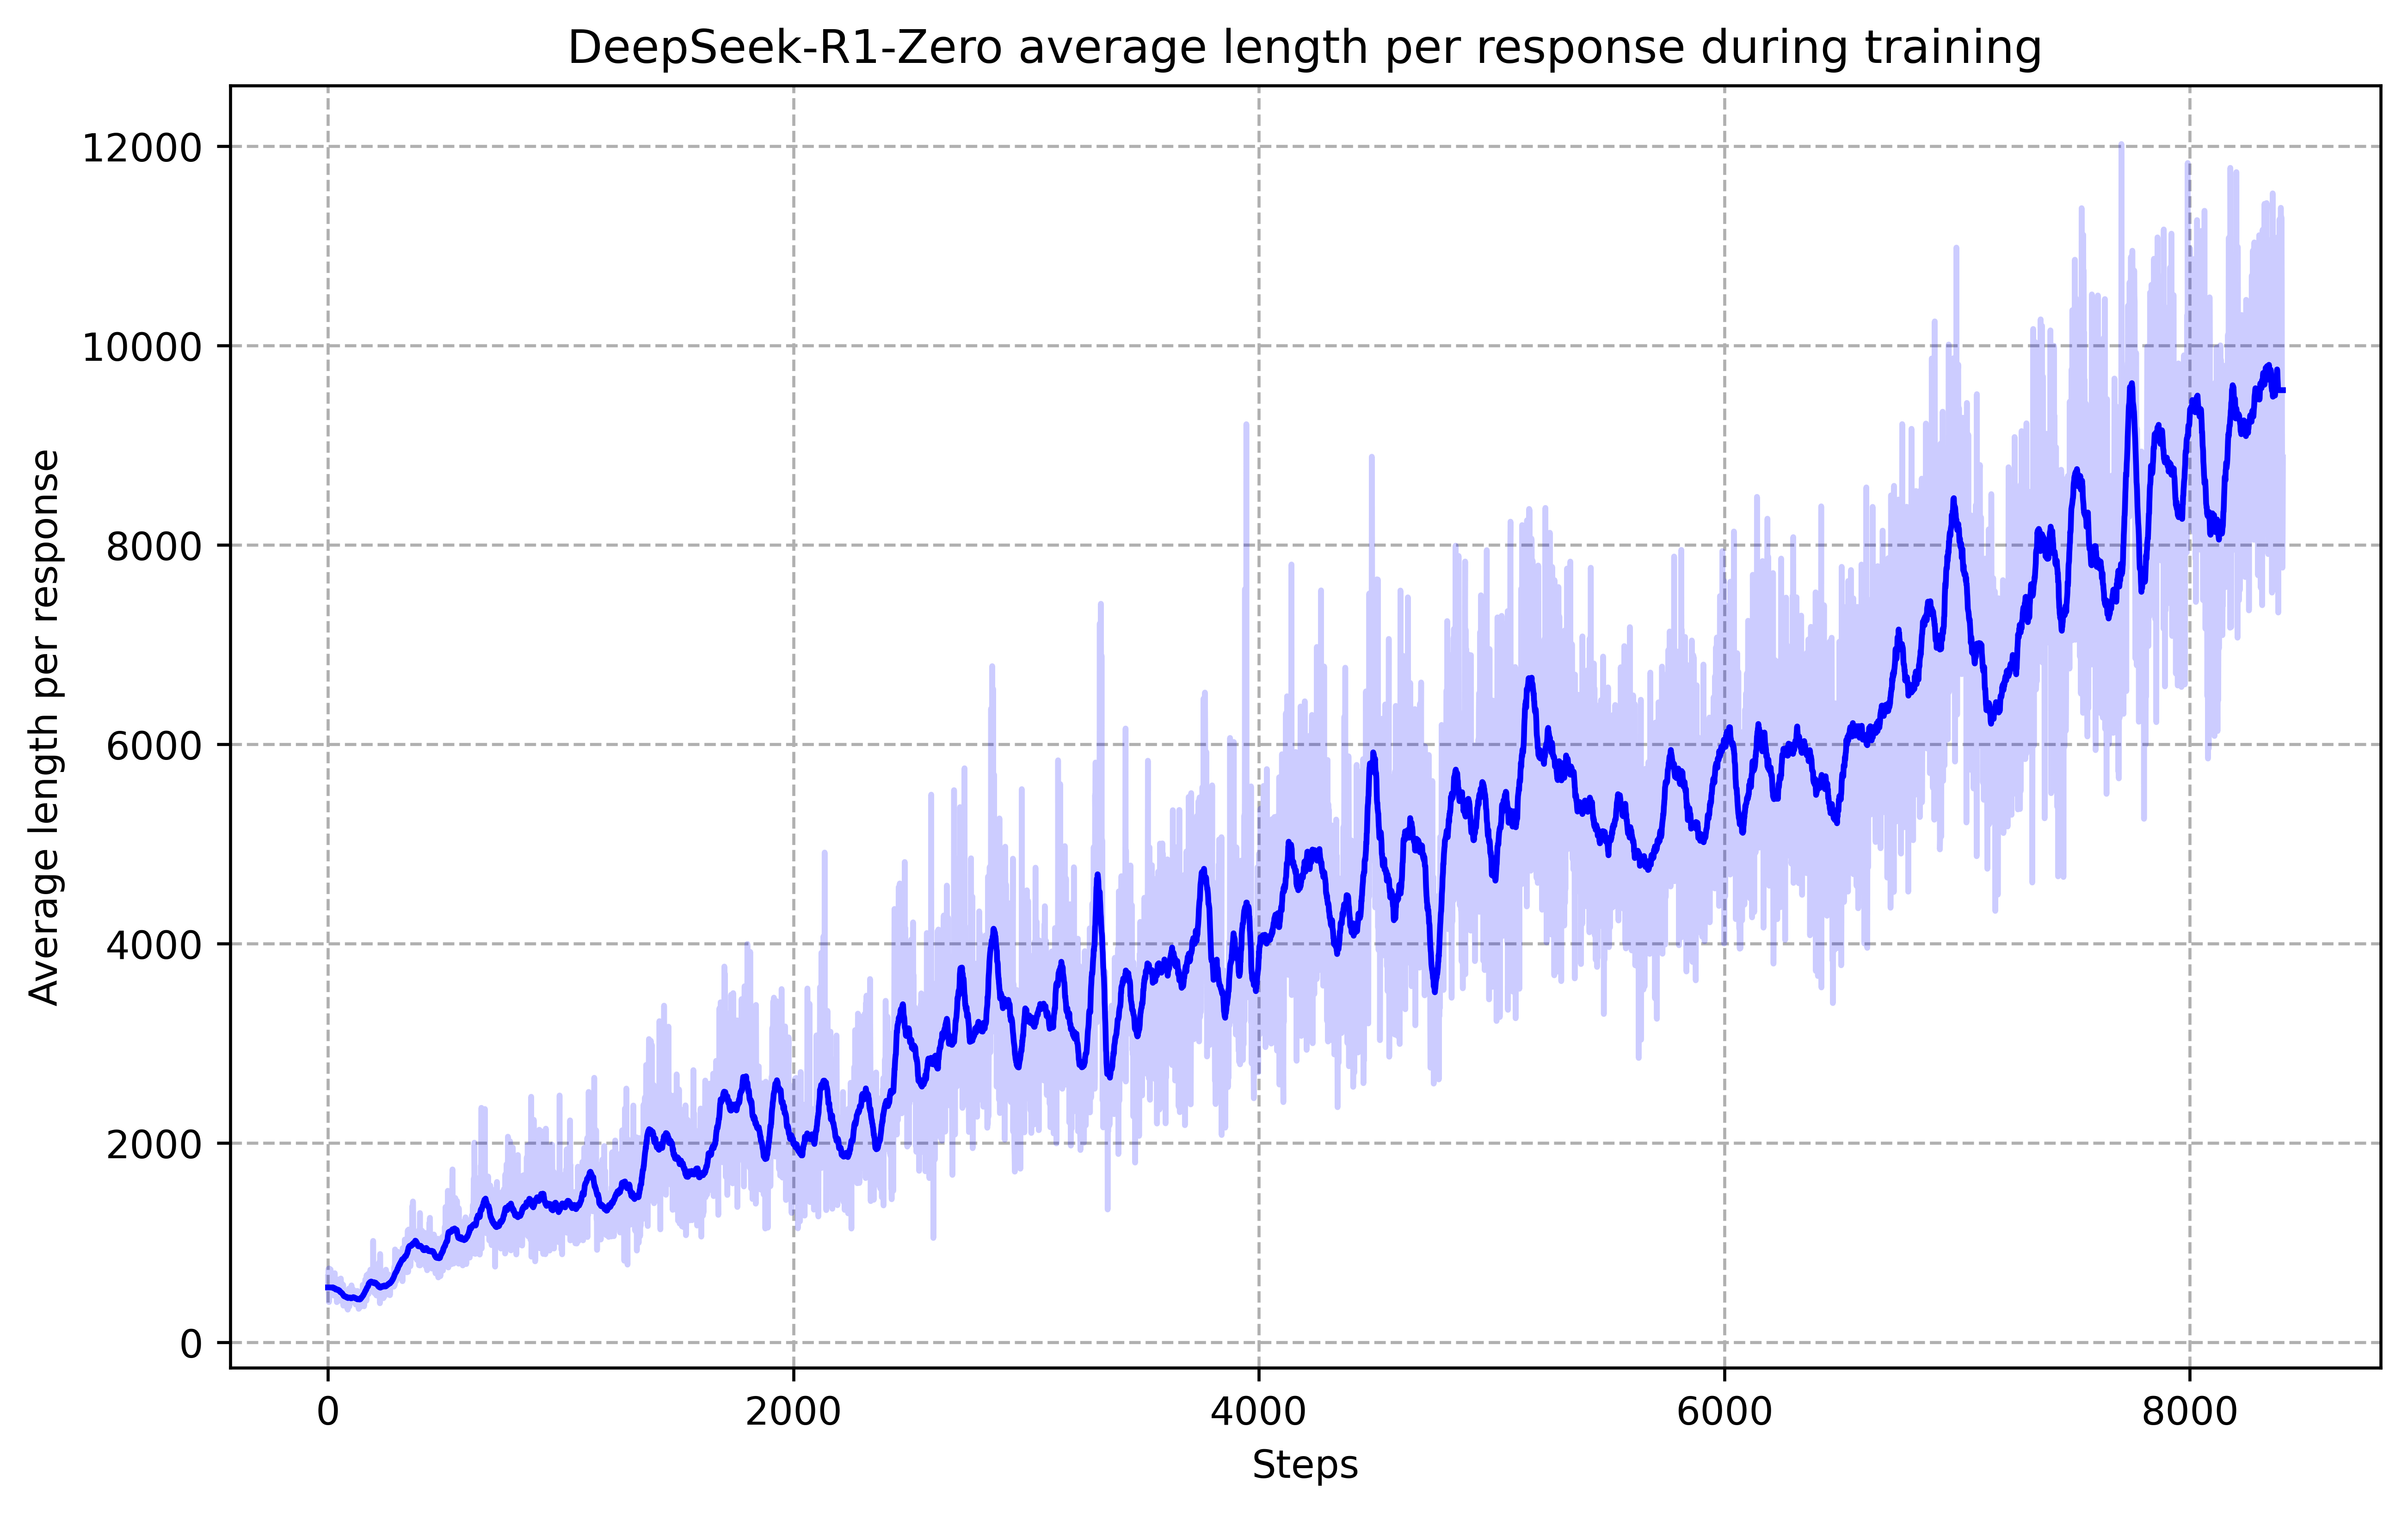
\includegraphics[width=0.75\linewidth]{figures/plot_length.png}
    \caption{The average response length of \dsro{} on the training set during the RL process. \dsro{} naturally learns to solve reasoning tasks with more thinking time.}
    \label{fig:zero-training-length}
\end{figure}

\paragraph{Self-evolution Process of \dsro{}}
The self-evolution process of \dsro{} is a fascinating demonstration of how RL can drive a model to improve its reasoning capabilities autonomously. By initiating RL directly from the base model, we can closely monitor the model's progression without the influence of the supervised fine-tuning stage. This approach provides a clear view of how the model evolves over time, particularly in terms of its ability to handle complex reasoning tasks.

As depicted in Figure \ref{fig:zero-training-length}, the thinking time of \dsro{} shows consistent improvement throughout the training process. This improvement is not the result of external adjustments but rather an intrinsic development within the model. \dsro{} naturally acquires the ability to solve increasingly complex reasoning tasks by leveraging extended test-time computation. This computation ranges from generating hundreds to thousands of reasoning tokens, allowing the model to explore and refine its thought processes in greater depth.

One of the most remarkable aspects of this self-evolution is the emergence of sophisticated behaviors as the test-time computation increases. Behaviors such as reflection—where the model revisits and reevaluates its previous steps—and the exploration of alternative approaches to problem-solving arise spontaneously. These behaviors are not explicitly programmed but instead emerge as a result of the model's interaction with the reinforcement learning environment. This spontaneous development significantly enhances \dsro{}'s reasoning capabilities, enabling it to tackle more challenging tasks with greater efficiency and accuracy.

\paragraph{Aha Moment of \dsro{}}
A particularly intriguing phenomenon observed during the training of \dsro{} is the occurrence of an ``aha moment''. This moment, as illustrated in Table \ref{tab:aha_moment}, occurs in an intermediate version of the model. During this phase, \dsro{} learns to allocate more thinking time to a problem by reevaluating its initial approach. This behavior is not only a testament to the model's growing reasoning abilities but also a captivating example of how reinforcement learning can lead to unexpected and sophisticated outcomes.

This moment is not only an ``aha moment'' for the model but also for the researchers observing its behavior. It underscores the power and beauty of reinforcement learning: rather than explicitly teaching the model on how to solve a problem, we simply provide it with the right incentives, and it autonomously develops advanced problem-solving strategies.
The ``aha moment'' serves as a powerful reminder of the potential of RL to unlock new levels of intelligence in artificial systems, paving the way for more autonomous and adaptive models in the future.

\paragraph{Drawback of \dsro{}}
Although \dsro{} exhibits strong reasoning capabilities and autonomously develops unexpected and powerful reasoning behaviors, it faces several issues. For instance, \dsro{} struggles with challenges like poor readability, and language mixing. To make reasoning processes more readable and share them with the open community, we explore \dsri{}, a method that utilizes RL with human-friendly cold-start data.


\begin{table}[t]
\centering
\begin{tabular}{l}
\toprule 
Question: If \(a > 1\), then the sum of the real solutions of \(\sqrt{a - \sqrt{a + x}} = x\) is equal to \\
\midrule
Response: <think> \\
To solve the equation \(\sqrt{a - \sqrt{a + x}} = x\), let's start by squaring both $\cdots$ \\
$\left(\sqrt{a - \sqrt{a + x}}\right)^2 = x^2 \implies a - \sqrt{a + x} = x^2.$ \\
Rearrange to isolate the inner square root term: \\
$(a - x^2)^2 = a + x \implies a^2 - 2ax^2 + (x^2)^2 = a + x \implies x^4 - 2ax^2 - x + (a^2 - a) = 0$ \\
\ldots \\
\textcolor{red}{Wait, wait. Wait. That's an aha moment I can flag here}. \\
Let's reevaluate this step-by-step to identify if the correct sum can be $\cdots$ \\
We started with the equation: \\
$\sqrt{a - \sqrt{a + x}} = x$ \\
First, let's square both sides: \\
$a - \sqrt{a + x} = x^2 \implies \sqrt{a + x} = a - x^2$ \\
Next, I could square both sides again, treating the equation: 
$\cdots$
\\
\ldots \\
\hline
\end{tabular}
\caption{An interesting ``aha moment'' of an intermediate version of \dsro{}. The model learns to rethink using an anthropomorphic tone. This is also an aha moment for us, allowing us to witness the power and beauty of reinforcement learning.}
\label{tab:aha_moment}
\end{table}


\subsection{\dsri{}: Reinforcement Learning with Cold Start}
Inspired by the promising results of \dsro{}, two natural questions arise: 1) Can reasoning performance be further improved or convergence accelerated by incorporating a small amount of high-quality data as a cold start? 2) How can we train a user-friendly model that not only produces clear and coherent Chains of Thought (CoT) but also demonstrates strong general capabilities?
To address these questions, we design a pipeline to train \dsri{}. The pipeline consists of four stages, outlined as follows.


\subsubsection{Cold Start}
Unlike \dsro{}, to prevent the early unstable cold start phase of RL training from the base model, for DeepSeek-R1 we construct and collect a small amount of long CoT data to fine-tune the model as the initial RL actor.
To collect such data, we have explored several approaches: using few-shot prompting with a long CoT as an example, directly prompting models to generate detailed answers with reflection and verification, gathering \dsro{} outputs in a readable format, and refining the results through post-processing by human annotators.


In this work, we collect thousands of cold-start data to fine-tune the DeepSeek-V3-Base as the starting point for RL.
Compared to \dsro{}, the advantages of cold start data include:
\begin{itemize}[topsep=0pt]
    \item 
Readability: A key limitation of \dsro{} is that its content is often not suitable for reading. Responses may mix multiple languages or lack markdown formatting to highlight answers for users. In contrast, when creating cold-start data for \dsri{}, we design a readable pattern that includes a summary at the end of each response and filters out responses that are not reader-friendly. Here, we define the output format as |special\_token|<reasoning\_process>|special\_token|<summary>, where the reasoning process is the CoT for the query, and the summary is used to summarize the reasoning results. 

 \item 
Potential: By carefully designing the pattern for cold-start data with human priors, we observe better performance against \dsro{}. We believe the iterative training is a better way for reasoning models. 
\end{itemize}

\subsubsection{Reasoning-oriented Reinforcement Learning}
After fine-tuning DeepSeek-V3-Base on the cold start data, we apply the same large-scale reinforcement learning training process as employed in \dsro. This phase focuses on enhancing the model's reasoning capabilities, particularly in reasoning-intensive tasks such as coding, mathematics, science, and logic reasoning, which involve well-defined problems with clear solutions. During the training process, we observe that CoT often exhibits language mixing, particularly when RL prompts involve multiple languages. To mitigate the issue of language mixing, we introduce a language consistency reward during RL training, which is calculated as the proportion of target language words in the CoT. Although ablation experiments show that such alignment results in a slight degradation in the model's performance, this reward aligns with human preferences, making it more readable. Finally, we combine the accuracy of reasoning tasks and the reward for language consistency by directly summing them to form the final reward. We then apply RL training on the fine-tuned model until it achieves convergence on reasoning tasks.

\subsubsection{Rejection Sampling and Supervised Fine-Tuning}
When reasoning-oriented RL converges, we utilize the resulting checkpoint to collect SFT (Supervised Fine-Tuning) data for the subsequent round. Unlike the initial cold-start data, which primarily focuses on reasoning, this stage incorporates data from other domains to enhance the model's capabilities in writing, role-playing, and other general-purpose tasks. Specifically, we generate the data and fine-tune the model as described below.
\label{sec:method:r1:sft}


\paragraph{Reasoning data}
We curate reasoning prompts and generate reasoning trajectories by performing rejection sampling from the checkpoint from the above RL training.
In the previous stage, we only included data that could be evaluated using rule-based rewards. However, in this stage, we expand the dataset by incorporating additional data, some of which use a generative reward model by feeding the ground-truth and model predictions into DeepSeek-V3 for judgment.
Additionally, because the model output is sometimes chaotic and difficult to read, we have filtered out chain-of-thought with mixed languages, long parapraphs, and code blocks.
For each prompt, we sample multiple responses and retain only the correct ones. In total, we collect about 600k reasoning related training samples. 

\paragraph{Non-Reasoning data}
For non-reasoning data, such as writing, factual QA, self-cognition, and translation, we adopt the DeepSeek-V3 pipeline and reuse portions of the SFT dataset of DeepSeek-V3. For certain non-reasoning tasks, we call DeepSeek-V3 to generate a potential chain-of-thought before answering the question by prompting. However, for simpler queries, such as ``hello'' we do not provide a CoT in response.
In the end, we collected a total of approximately 200k training samples that are unrelated to reasoning.


We fine-tune DeepSeek-V3-Base for two epochs using the above curated dataset of about 800k samples.


\subsubsection{Reinforcement Learning for all Scenarios}

To further align the model with human preferences, we implement a secondary reinforcement learning stage aimed at improving the model's helpfulness and harmlessness while simultaneously refining its reasoning capabilities. Specifically, we train the model using a combination of reward signals and diverse prompt distributions.
For reasoning data, we adhere to the methodology outlined in \dsro, which utilizes rule-based rewards to guide the learning process in math, code, and logical reasoning domains. 
For general data, we resort to reward models to capture human preferences in complex and nuanced scenarios. We build upon the DeepSeek-V3 pipeline and adopt a similar distribution of preference pairs and training prompts. For helpfulness, we focus exclusively on the final summary, ensuring that the assessment emphasizes the utility and relevance of the response to the user while minimizing interference with the underlying reasoning process. For harmlessness, we evaluate the entire response of the model, including both the reasoning process and the summary, to identify and mitigate any potential risks, biases, or harmful content that may arise during the generation process. 
Ultimately, the integration of reward signals and diverse data distributions enables us to train a model that excels in reasoning while prioritizing helpfulness and harmlessness.


\subsection{Distillation: Empower Small Models with Reasoning Capability }

To equip more efficient smaller models with reasoning capabilities like DeepSeek-R1, we directly fine-tuned open-source models like Qwen \citep{qwen2_5} and Llama \citep{llama3_1_405b} using the 800k samples curated with DeepSeek-R1, as detailed in \S \ref{sec:method:r1:sft}.
Our findings indicate that this straightforward distillation method significantly enhances the reasoning abilities of smaller models.
The base models we use here are Qwen2.5-Math-1.5B, Qwen2.5-Math-7B, Qwen2.5-14B, Qwen2.5-32B, Llama-3.1-8B, and Llama-3.3-70B-Instruct. We select Llama-3.3 because its reasoning capability is slightly better than that of Llama-3.1.

For distilled models, we apply only SFT and do not include an RL stage, even though incorporating RL could substantially boost model performance. Our primary goal here is to demonstrate the effectiveness of the distillation technique, leaving the exploration of the RL stage to the broader research community.

\section{Experiment}

\paragraph{Benchmarks} We evaluate models on MMLU \citep{mmlu}, MMLU-Redux \citep{mmlu_redux}, MMLU-Pro \citep{mmlu_pro}, C-Eval \citep{ceval}, and CMMLU \citep{cmmlu}, IFEval~\citep{IFeval}, FRAMES~\citep{frames}, GPQA Diamond ~\citep{gpqa}, SimpleQA~\citep{simpleqa}, C-SimpleQA~\citep{csimpleqa}, SWE-Bench Verified~\citep{swe_verified}, Aider~\footnote{\url{https://aider.chat}}, LiveCodeBench~\citep{livecodebench} (2024-08 -- 2025-01), Codeforces~\footnote{\url{https://codeforces.com}}, Chinese National High School Mathematics Olympiad (CNMO 2024)\footnote{\url{https://www.cms.org.cn/Home/comp/comp/cid/12.html}}, and American Invitational Mathematics Examination 2024 (AIME 2024)~\citep{AIME2024}. 
In addition to standard benchmarks, we also evaluate our models on open-ended generation tasks using LLMs as judges. 
Specifically, we adhere to the original configurations of AlpacaEval 2.0~\citep{alpaca2.0} and Arena-Hard~\citep{li2024crowdsourced}, which leverage GPT-4-Turbo-1106 as judges for pairwise comparisons. Here, we only feed the final summary to evaluation to avoid the length bias. 
For distilled models, we report representative results on AIME 2024, MATH-500, GPQA Diamond, Codeforces, and LiveCodeBench.


\paragraph{Evaluation Prompts} Following the setup in DeepSeek-V3, standard benchmarks such as MMLU, DROP, GPQA Diamond, and SimpleQA are evaluated using prompts from the simple-evals framework. For MMLU-Redux, we adopt the Zero-Eval prompt format~\citep{Lin_ZeroEval_A_Unified_2024} in a zero-shot setting. In terms of MMLU-Pro, C-Eval and CLUE-WSC, since the original prompts are few-shot, we slightly modify the prompt to the zero-shot setting. The CoT in few-shot may hurt the performance of  \dsri{}. 
Other datasets follow their original evaluation protocols with default prompts provided by their creators. 
For code and math benchmarks, the HumanEval-Mul dataset covers eight mainstream programming languages (Python, Java, C++, C\#, JavaScript, TypeScript, PHP, and Bash). 
Model performance on LiveCodeBench is evaluated using  CoT format, with data collected between August 2024 and January 2025. The Codeforces dataset is evaluated using problems from 10 Div.2 contests along with expert-crafted test cases, after which the expected ratings and percentages of competitors are calculated. SWE-Bench verified results are obtained via the agentless framework~\citep{agentless}. AIDER-related benchmarks are measured using a "diff" format.
\dsri{} outputs are capped at a maximum of 32,768 tokens for each benchmark.


\paragraph{Baselines} We conduct comprehensive evaluations against several strong baselines, including DeepSeek-V3, Claude-Sonnet-3.5-1022, GPT-4o-0513, OpenAI-o1-mini, and OpenAI-o1-1217. Since accessing the OpenAI-o1-1217 API is challenging in mainland China, we report its performance based on official reports.
For distilled models, we also compare the open-source model QwQ-32B-Preview \citep{QwQ}.




\paragraph{Evaluation Setup}
We set the maximum generation length to 32,768 tokens for the models.
We found that using greedy decoding to evaluate long-output reasoning models results in higher repetition rates and significant variability across different checkpoints.
Therefore, we default to pass@$k$ evaluation \citep{codex} and report pass@1 using a non-zero temperature.
Specifically, we use a sampling temperature of $0.6$ and a top-$p$ value of $0.95$ to generate $k$ responses (typically between $4$ and $64$, depending on the test set size) for each question. Pass@1 is then calculated as
\[
\text{pass@1} = \frac{1}{k} \sum_{i=1}^{k} p_i,
\]
where $p_i$ denotes the correctness of the $i$-th response. This method provides more reliable performance estimates.
For AIME 2024, we also report consensus (majority vote) results \citep{wang2022self} using $64$ samples, denoted as $\text{cons}@64$.


\subsection{\dsri{} Evaluation}

\begin{table}[h]
    \centering
    \footnotesize
    \setlength{\tabcolsep}{1.9pt}
    \begin{tabular}{@{}c l | c  c  c | c c |c c@{}}
    \toprule
    & \multirow{2}{*}{\centering \textbf{Benchmark {\tiny (Metric)}}}  & \textbf{Claude-3.5-}  & \textbf{GPT-4o}& \textbf{DeepSeek} & \textbf{OpenAI} & \textbf{OpenAI} & \textbf{DeepSeek}\\
    & & \textbf{Sonnet-1022}  & \textbf{0513} & \textbf{V3} & \textbf{o1-mini}& \textbf{o1-1217} &\textbf{R1} \\
    \midrule
    & Architecture &-&- & MoE &-&-& MoE \\
    & \# Activated Params& -&-& 37B&-&- & 37B \\
    & \# Total Params &-&-& 671B&-&- & 671B \\
    \midrule
    \multirow{10}{*}{English}& MMLU {\tiny (Pass@1)} & 88.3&87.2 & 88.5 & 85.2 & \textbf{91.8} & 90.8\\
     & MMLU-Redux {\tiny (EM)}& 88.9& 88.0 & 89.1 & 86.7&- & \textbf{92.9} \\
    & MMLU-Pro {\tiny (EM)}  & 78.0 & 72.6 & 75.9 & 80.3 &-& \textbf{84.0} \\
    & DROP {\tiny (3-shot F1)}  & 88.3 & 83.7 & 91.6 & 83.9 & 90.2 & \textbf{92.2}\\
    & IF-Eval {\tiny (Prompt Strict)}  & \textbf{86.5} & 84.3 & 86.1 & 84.8&- & 83.3 \\
    & GPQA Diamond {\tiny (Pass@1)}& 65.0 & 49.9 & 59.1 & 60.0 & \textbf{75.7} & 71.5&  \\
    & SimpleQA {\tiny (Correct)} & 28.4 & 38.2& 24.9 & 7.0 & \textbf{47.0} & 30.1 \\
     & FRAMES {\tiny (Acc.)}  & 72.5 & 80.5 & 73.3 & 76.9 & -&\textbf{82.5}\\
      & AlpacaEval2.0 {\tiny (LC-winrate)}  & 52.0 &  51.1 & 70.0 & 57.8 & - & \textbf{87.6}\\
       & ArenaHard {\tiny (GPT-4-1106)}  & 85.2 & 80.4 & 85.5 & 92.0 & - & \textbf{92.3}\\
    \midrule
    \multirow{4}{*}{Code} & LiveCodeBench {\tiny (Pass@1-COT)} & 38.9 & 32.9 & 36.2 & 53.8 & 63.4 & \textbf{65.9} \\
    & Codeforces {\tiny (Percentile)}& 20.3 & 23.6 & 58.7 & 93.4 & \textbf{96.6} & 96.3 \\
    & Codeforces {\tiny (Rating)}& 717 & 759 & 1134 & 1820 & \textbf{2061} & 2029 \\
    & SWE Verified {\tiny (Resolved)} & \textbf{50.8}&38.8&42.0 & 41.6 & 48.9 & 49.2\\
    & Aider-Polyglot {\tiny (Acc.)} & 45.3&16.0& 49.6 & 32.9 & \textbf{61.7}&53.3\\
    \midrule
    \multirow{3}{*}{Math} & AIME 2024 {\tiny (Pass@1)}  & 16.0 & 9.3 & 39.2 & 63.6 & 79.2 & \textbf{79.8} \\
    & MATH-500 {\tiny (Pass@1)} &78.3 & 74.6&90.2 & 90.0 & 96.4 & \textbf{97.3} \\
    & CNMO 2024 {\tiny (Pass@1)} & 13.1 & 10.8 &43.2 & 67.6 & - & \textbf{78.8} \\
    \midrule
    \multirow{3}{*}{Chinese} & CLUEWSC {\tiny (EM)}&  85.4 & 87.9 & 90.9 & 89.9 & - &\textbf{92.8}\\
    & C-Eval {\tiny (EM)} & 76.7 & 76.0 & 86.5 & 68.9 & - & \textbf{91.8}\\
     & C-SimpleQA {\tiny (Correct)}  & 55.4 & 58.7 & \textbf{68.0} & 40.3 & -& 63.7 \\
    \bottomrule
    \end{tabular}
    \caption{ Comparison between \dsri{} and other representative models. 
    }
    \label{tab:main}
\end{table}

For education-oriented knowledge benchmarks such as MMLU, MMLU-Pro, and GPQA Diamond, \dsri{} demonstrates superior performance compared to DeepSeek-V3. This improvement is primarily attributed to enhanced accuracy in STEM-related questions, where significant gains are achieved through large-scale reinforcement learning. Additionally, \dsri{} excels on FRAMES, a long-context-dependent QA task, showcasing its strong document analysis capabilities. This highlights the potential of reasoning models in AI-driven search and data analysis tasks. On the factual benchmark SimpleQA, \dsri{} outperforms DeepSeek-V3, demonstrating its capability in handling fact-based queries. A similar trend is observed where OpenAI-o1 surpasses GPT-4o on this benchmark. However, \dsri{} performs worse than DeepSeek-V3 on the Chinese SimpleQA benchmark, primarily due to its tendency to refuse answering certain queries after safety RL. Without safety RL, \dsri{} could achieve an accuracy of over 70\%.


\dsri{} also delivers impressive results on IF-Eval, a benchmark designed to assess a model's ability to follow format instructions. These improvements can be linked to the inclusion of instruction-following data during the final stages of supervised fine-tuning (SFT) and RL training. Furthermore, remarkable performance is observed on AlpacaEval2.0 and ArenaHard, indicating \dsri{}’s strengths in writing tasks and open-domain question answering. Its significant outperformance of DeepSeek-V3 underscores the generalization benefits of large-scale RL, which not only boosts reasoning capabilities but also improves performance across diverse domains.
Moreover, the summary lengths generated by \dsri{} are concise, with an average of 689 tokens on ArenaHard and 2,218 characters on AlpacaEval 2.0. This indicates that \dsri{} avoids introducing length bias during GPT-based evaluations, further solidifying its robustness across multiple tasks.

On math tasks, \dsri{} demonstrates performance on par with OpenAI-o1-1217, surpassing other models by a large margin. A similar trend is observed on coding algorithm tasks, such as LiveCodeBench and Codeforces, where reasoning-focused models dominate these benchmarks. On engineering-oriented coding tasks, OpenAI-o1-1217 outperforms \dsri{} on Aider but achieves comparable performance on SWE Verified. We believe the engineering performance of \dsri{} will improve in the next version, as the amount of related RL training data currently remains very limited.


\subsection{Distilled Model Evaluation}
\label{sec:distilled_model_evaluation}
\begin{table}[h]
    \centering
    \resizebox{\linewidth}{!}{
    \begin{tabular}{@{}l *{6}{c} @{}}
    \toprule
    \multirow{3}{*}{\centering\textbf{Model}} & \multicolumn{2}{c}{\multirow{2}{*}{\textbf{AIME 2024}}} & \multirow{2}{*}{\textbf{MATH-500}} & \textbf{GPQA} & \textbf{LiveCode} & \multirow{2}{*}{\textbf{CodeForces}} \\
    &  &  &  & \textbf{Diamond} & \textbf{Bench} \\
    \cmidrule(lr){2-3}
     & pass@1 & cons@64 & pass@1 & pass@1 & pass@1 & rating \\
    \midrule
    \textbf{GPT-4o-0513} & 9.3 & 13.4 & 74.6  & 49.9 & 32.9 &  759\\
    \textbf{Claude-3.5-Sonnet-1022} & 16.0 & 26.7 & 78.3  & 65.0 & 38.9 &  717\\
    \textbf{OpenAI-o1-mini} & 63.6 & 80.0 & 90.0 &  60.0 & 53.8 &  \textbf{1820}\\
    \textbf{QwQ-32B-Preview} & 50.0 & 60.0 & 90.6 & 54.5 & 41.9 &  1316 \\
    \midrule
    \textbf{DeepSeek-R1-Distill-Qwen-1.5B} & 28.9 & 52.7 & 83.9 & 33.8 & 16.9 & 954 \\
    \textbf{DeepSeek-R1-Distill-Qwen-7B} & 55.5 & 83.3 & 92.8 & 49.1 & 37.6 & 1189 \\
    \textbf{DeepSeek-R1-Distill-Qwen-14B} & 69.7 & 80.0 & 93.9 &  59.1 & 53.1 & 1481 \\
    \textbf{DeepSeek-R1-Distill-Qwen-32B} & \textbf{72.6} & {83.3} & {94.3} & {62.1} & {57.2} & 1691 \\
    \textbf{DeepSeek-R1-Distill-Llama-8B} & 50.4 & 80.0 & 89.1 & 49.0 & 39.6 & 1205 \\
    \textbf{DeepSeek-R1-Distill-Llama-70B} & 70.0 & \textbf{86.7} & \textbf{94.5} & \textbf{65.2} & \textbf{57.5} & 1633 \\
    \bottomrule
    \end{tabular}
    }
    \caption{DeepSeek-R1 蒸馏模型与其他可比较模型在推理相关基准上的比较。}
    \label{tab:distill}
\end{table}


As shown in Table \ref{tab:distill}, simply distilling DeepSeek-R1's outputs enables the efficient DeepSeek-R1-7B (i.e., DeepSeek-R1-Distill-Qwen-7B, abbreviated similarly below) to outperform non-reasoning models like GPT-4o-0513 across the board.
DeepSeek-R1-14B surpasses QwQ-32B-Preview on all evaluation metrics, while DeepSeek-R1-32B and DeepSeek-R1-70B significantly exceed o1-mini on most benchmarks.
These results demonstrate the strong potential of distillation.
Additionally, we found that applying RL to these distilled models yields significant further gains. We believe this warrants further exploration and therefore present only the results of the simple SFT-distilled models here.


\section{Discussion}
\subsection{Distillation v.s. Reinforcement Learning}
\begin{table}[h]
    \centering
    \resizebox{\linewidth}{!}{
    \begin{tabular}{@{}l *{6}{c} @{}}
    \toprule
    \multirow{3}{*}{\centering\textbf{Model}} & \multicolumn{2}{c}{\textbf{AIME 2024}} & \textbf{MATH-500} & \textbf{GPQA Diamond} & \textbf{LiveCodeBench}  \\

    \cmidrule(lr){2-3}
     & pass@1 & cons@64 & pass@1& pass@1 & pass@1 \\
    \midrule
    \textbf{QwQ-32B-Preview} & 50.0 & 60.0 & 90.6 & 54.5 & 41.9  \\
    \textbf{DeepSeek-R1-Zero-Qwen-32B} & 47.0 & 60.0 & 91.6  & 55.0 & 40.2  \\
    \textbf{DeepSeek-R1-Distill-Qwen-32B} & \bf{72.6} & \bf{83.3} & \bf{94.3}  & \bf{62.1} & \bf{57.2}\\
    \bottomrule
    \end{tabular}
    }
    \caption{\centering 蒸馏模型和 RL 模型在推理相关基准上的比较。}
    \label{tab:distill_vs_rl}
\end{table}


In Section \ref{sec:distilled_model_evaluation}, we can see that by distilling DeepSeek-R1, the small model can achieve impressive results. However, there is still one question left: can the model achieve comparable performance through the large-scale RL training discussed in the paper without distillation?


To answer this question, we conduct large-scale RL training on Qwen-32B-Base using math, code, and STEM data, training for over 10K steps, resulting in DeepSeek-R1-Zero-Qwen-32B. The experimental results, shown in Table \ref{tab:distill_vs_rl}, demonstrate that the 32B base model, after large-scale RL training, achieves performance on par with QwQ-32B-Preview. However, DeepSeek-R1-Distill-Qwen-32B, which is distilled from DeepSeek-R1,  performs significantly better than DeepSeek-R1-Zero-Qwen-32B across all benchmarks.

Therefore, we can draw two conclusions: First, distilling more powerful models into smaller ones yields excellent results, whereas smaller models relying on the large-scale RL mentioned in this paper require enormous computational power and may not even achieve the performance of distillation. Second, while distillation strategies are both economical and effective, advancing beyond the boundaries of intelligence may still require more powerful base models and larger-scale reinforcement learning.

\subsection{Unsuccessful Attempts}
In the early stages of developing \dsri{}, we also encountered failures and setbacks along the way. We share our failure experiences here to provide insights, but this does not imply that these approaches are incapable of developing effective reasoning models.

\paragraph{Process Reward Model (PRM)}
PRM is a reasonable method to guide the model toward better approaches for solving reasoning tasks~\citep{uesato2022solving, lightman2023let,mathshepherd}. However, in practice, PRM has three main limitations that may hinder its ultimate success. First, it is challenging to explicitly define a fine-grain step in general reasoning. 
Second, determining whether the current intermediate step is correct is a challenging task. Automated annotation using models may not yield satisfactory results, while manual annotation is not conducive to scaling up.
Third, once a model-based PRM is introduced, it inevitably leads to reward hacking~\citep{gao2022scalinglawsrewardmodel},  and retraining the reward model needs additional training resources and it complicates the whole training pipeline. In conclusion, while PRM demonstrates a good ability to rerank the top-N responses generated by the model or assist in guided search~\citep{snell2024scalingllmtesttimecompute}, its advantages are limited compared to the additional computational overhead it introduces during the large-scale reinforcement learning process in our experiments.

\paragraph{Monte Carlo Tree Search (MCTS)}
Inspired by AlphaGo~\citep{alphago} and AlphaZero~\citep{alphazero}, we explored using Monte Carlo Tree Search (MCTS) to enhance test-time compute scalability. This approach involves breaking answers into smaller parts to allow the model to explore the solution space systematically. To facilitate this, we prompt the model to generate multiple tags that correspond to specific reasoning steps necessary for the search. For training, we first use collected prompts to find answers via MCTS guided by a pre-trained value model. Subsequently, we use the resulting question-answer pairs to train both the actor model and the value model, iteratively refining the process.

However, this approach encounters several challenges when scaling up the training. First, unlike chess, where the search space is relatively well-defined, token generation presents an exponentially larger search space. To address this, we set a maximum extension limit for each node, but this can lead to the model getting stuck in local optima. Second, the value model directly influences the quality of generation since it guides each step of the search process. Training a fine-grained value model is inherently difficult, which makes it challenging for the model to iteratively improve. While AlphaGo's core success relied on training a value model to progressively enhance its performance, this principle proves difficult to replicate in our setup due to the complexities of token generation.

In conclusion, while MCTS can improve performance during inference when paired with a pre-trained value model, iteratively boosting model performance through self-search remains a significant challenge.




\section{Conclusion, Limitations, and Future Work}

In this work, we share our journey in enhancing model reasoning abilities through reinforcement learning. \dsro{} represents a pure RL approach without relying on cold-start data, achieving strong performance across various tasks. \dsri{} is more powerful, leveraging cold-start data alongside iterative RL fine-tuning. Ultimately, \dsri{} achieves performance comparable to OpenAI-o1-1217 on a range of tasks.

We further explore distillation the reasoning capability to small dense models. We use \dsri{} as the teacher model to generate 800K training samples, and fine-tune several small dense models. The results are promising: DeepSeek-R1-Distill-Qwen-1.5B outperforms GPT-4o and Claude-3.5-Sonnet on math benchmarks with 28.9\% on AIME and 83.9\% on MATH. Other dense models also achieve impressive results, significantly outperforming other instruction-tuned models based on the same underlying checkpoints.

In the future, we plan to invest in research across the following directions for \dsri{}.
\begin{itemize}[topsep=0pt]
    \item \textbf{General Capability:}
  Currently, the capabilities of \dsri{} fall short of DeepSeek-V3 in tasks such as function calling, multi-turn, complex role-playing, and JSON output. Moving forward, we plan to explore how long CoT can be leveraged to enhance tasks in these fields.
    \item \textbf{Language Mixing:}
\dsri{} is currently optimized for Chinese and English, which may result in language mixing issues when handling queries in other languages. For instance, \dsri{} might use English for reasoning and responses, even if the query is in a language other than English or Chinese. We aim to address this limitation in future updates.
 \item \textbf{Prompting Engineering:} When evaluating \dsri{}, we observe that it is sensitive to prompts. Few-shot prompting consistently degrades its performance. Therefore, we recommend users directly describe the problem and specify the output format using a zero-shot setting for optimal results.
\item  \textbf{Software Engineering Tasks:}
Due to the long evaluation times, which impact the efficiency of the RL process, large-scale RL has not been applied extensively in software engineering tasks. As a result, DeepSeek-R1 has not demonstrated a huge improvement over DeepSeek-V3 on software engineering benchmarks. Future versions will address this by implementing rejection sampling on software engineering data or incorporating asynchronous evaluations during the RL process to improve efficiency.
    
\end{itemize}

\bibliography{main}

\newpage
\appendix

\section*{Appendix}

\section{Contributions and Acknowledgments}

\definecolor{damaiblue}{RGB}{0, 0, 100}
\definecolor{damaigreen}{RGB}{0, 100, 0}
\definecolor{damaired}{RGB}{100, 0, 0}

\begin{multicols}{2} %
\noindent
\textbf{\color{damaired} Core Contributors} \\
\color{damaired} Daya Guo \\
\color{damaired} Dejian Yang \\
\color{damaired} Haowei Zhang \\
\color{damaired} Junxiao Song \\
\color{damaired} Ruoyu Zhang \\
\color{damaired} Runxin Xu \\
\color{damaired} Qihao Zhu \\
\color{damaired} Shirong Ma \\
\color{damaired} Peiyi Wang \\
\color{damaired} Xiao Bi \\
\color{damaired} Xiaokang Zhang \\
\color{damaired} Xingkai Yu \\
\color{damaired} Yu Wu \\
\color{damaired} Z.F. Wu \\
\color{damaired} Zhibin Gou \\
\color{damaired} Zhihong Shao \\
\color{damaired} Zhuoshu Li \\
\color{damaired} Ziyi Gao \\

\noindent
\textbf{\color{damaiblue} Contributors} \\
\color{damaiblue} 
\color{damaiblue} Aixin Liu \\
\color{damaiblue} Bing Xue \\
\color{damaiblue} Bingxuan Wang \\
\color{damaiblue} Bochao Wu \\
\color{damaiblue} Bei Feng \\
\color{damaiblue} Chengda Lu \\
\color{damaiblue} Chenggang Zhao \\
\color{damaiblue} Chengqi Deng \\
\color{damaiblue} Chong Ruan \\
\color{damaiblue} Damai Dai \\
\color{damaiblue} Deli Chen \\
\color{damaiblue} Dongjie Ji \\
\color{damaiblue} Erhang Li \\
\color{damaiblue} Fangyun Lin \\
\color{damaiblue} Fucong Dai \\
\color{damaiblue} Fuli Luo* \\
\color{damaiblue} Guangbo Hao \\
\color{damaiblue} Guanting Chen \\
\color{damaiblue} Guowei Li \\
\color{damaiblue} H. Zhang \\
\color{damaiblue} Hanwei Xu \\
\color{damaiblue} Honghui Ding \\
\color{damaiblue} Huazuo Gao \\
\color{damaiblue} Hui Qu \\
\color{damaiblue} Hui Li \\
\color{damaiblue} Jianzhong Guo \\
\color{damaiblue} Jiashi Li \\
\color{damaiblue} Jingchang Chen \\
\color{damaiblue} Jingyang Yuan \\
\color{damaiblue} Jinhao Tu \\
\color{damaiblue} Junjie Qiu \\
\color{damaiblue} Junlong Li \\
\color{damaiblue} J.L. Cai \\
\color{damaiblue} Jiaqi Ni \\
\color{damaiblue} Jian Liang \\
\color{damaiblue} Jin Chen \\
\color{damaiblue} Kai Dong \\
\color{damaiblue} Kai Hu* \\
\color{damaiblue} Kaichao You \\
\color{damaiblue} Kaige Gao \\
\color{damaiblue} Kang Guan \\
\color{damaiblue} Kexin Huang \\
\color{damaiblue} Kuai Yu \\
\color{damaiblue} Lean Wang \\
\color{damaiblue} Lecong Zhang \\
\color{damaiblue} Liang Zhao \\
\color{damaiblue} Litong Wang \\
\color{damaiblue} Liyue Zhang \\
\color{damaiblue} Lei Xu \\
\color{damaiblue} Leyi Xia \\
\color{damaiblue} Mingchuan Zhang \\
\color{damaiblue} Minghua Zhang \\
\color{damaiblue} Minghui Tang \\
\color{damaiblue} Mingxu Zhou \\
\color{damaiblue} Meng Li \\
\color{damaiblue} Miaojun Wang \\
\color{damaiblue} Mingming Li \\
\color{damaiblue} Ning Tian \\
\color{damaiblue} Panpan Huang \\
\color{damaiblue} Peng Zhang \\
\color{damaiblue} Qiancheng Wang \\
\color{damaiblue} Qinyu Chen \\
\color{damaiblue} Qiushi Du \\
\color{damaiblue} Ruiqi Ge* \\
\color{damaiblue} Ruisong Zhang \\
\color{damaiblue} Ruizhe Pan \\
\color{damaiblue} Runji Wang \\
\color{damaiblue} R.J. Chen \\
\color{damaiblue} R.L. Jin \\
\color{damaiblue} Ruyi Chen \\
\color{damaiblue} Shanghao Lu \\
\color{damaiblue} Shangyan Zhou \\
\color{damaiblue} Shanhuang Chen \\
\color{damaiblue} Shengfeng Ye \\
\color{damaiblue} Shiyu Wang \\
\color{damaiblue} Shuiping Yu \\
\color{damaiblue} Shunfeng Zhou \\
\color{damaiblue} Shuting Pan \\
\color{damaiblue} S.S. Li \\
\color{damaiblue} Shuang Zhou \\
\color{damaiblue} Shaoqing Wu \\
\color{damaiblue} Shengfeng Ye \\
\color{damaiblue} Tao Yun \\
\color{damaiblue} Tian Pei \\
\color{damaiblue} Tianyu Sun \\
\color{damaiblue} T. Wang \\
\color{damaiblue} Wangding Zeng \\
\color{damaiblue} Wen Liu \\
\color{damaiblue} Wenfeng Liang \\
\color{damaiblue} Wenjun Gao \\
\color{damaiblue} Wenqin Yu* \\
\color{damaiblue} Wentao Zhang \\
\color{damaiblue} W.L. Xiao \\
\color{damaiblue} Wei An \\
\color{damaiblue} Xiaodong Liu \\
\color{damaiblue} Xiaohan Wang \\
\color{damaiblue} Xiaokang Chen \\
\color{damaiblue} Xiaotao Nie \\
\color{damaiblue} Xin Cheng \\
\color{damaiblue} Xin Liu \\
\color{damaiblue} Xin Xie \\
\color{damaiblue} Xingchao Liu \\
\color{damaiblue} Xinyu Yang \\
\color{damaiblue} Xinyuan Li \\
\color{damaiblue} Xuecheng Su \\
\color{damaiblue} Xuheng Lin \\
\color{damaiblue} X.Q. Li \\
\color{damaiblue} Xiangyue Jin \\
\color{damaiblue} Xiaojin Shen \\
\color{damaiblue} Xiaosha Chen \\
\color{damaiblue} Xiaowen Sun \\
\color{damaiblue} Xiaoxiang Wang \\
\color{damaiblue} Xinnan Song \\
\color{damaiblue} Xinyi Zhou \\
\color{damaiblue} Xianzu Wang \\
\color{damaiblue} Xinxia Shan \\
\color{damaiblue} Y.K. Li \\
\color{damaiblue} Y.Q. Wang \\
\color{damaiblue} Y.X. Wei \\
\color{damaiblue} Yang Zhang \\
\color{damaiblue} Yanhong Xu \\
\color{damaiblue} Yao Li \\
\color{damaiblue} Yao Zhao \\
\color{damaiblue} Yaofeng Sun \\
\color{damaiblue} Yaohui Wang \\
\color{damaiblue} Yi Yu \\
\color{damaiblue} Yichao Zhang \\
\color{damaiblue} Yifan Shi \\
\color{damaiblue} Yiliang Xiong \\
\color{damaiblue} Ying He \\
\color{damaiblue} Yishi Piao \\
\color{damaiblue} Yisong Wang \\
\color{damaiblue} Yixuan Tan \\
\color{damaiblue} Yiyang Ma* \\
\color{damaiblue} Yiyuan Liu \\
\color{damaiblue} Yongqiang Guo \\
\color{damaiblue} Yuan Ou \\
\color{damaiblue} Yuduan Wang \\
\color{damaiblue} Yue Gong \\
\color{damaiblue} Yuheng Zou \\
\color{damaiblue} Yujia He \\
\color{damaiblue} Yunfan Xiong \\
\color{damaiblue} Yuxiang Luo \\
\color{damaiblue} Yuxiang You \\
\color{damaiblue} Yuxuan Liu \\
\color{damaiblue} Yuyang Zhou \\
\color{damaiblue} Y.X. Zhu \\
\color{damaiblue} Yanping Huang \\
\color{damaiblue} Yaohui Li \\
\color{damaiblue} Yi Zheng \\
\color{damaiblue} Yuchen Zhu \\
\color{damaiblue} Yunxian Ma \\
\color{damaiblue} Ying Tang \\
\color{damaiblue} Yukun Zha \\
\color{damaiblue} Yuting Yan \\
\color{damaiblue} Z.Z. Ren \\
\color{damaiblue} Zehui Ren \\
\color{damaiblue} Zhangli Sha \\
\color{damaiblue} Zhe Fu \\
\color{damaiblue} Zhean Xu \\
\color{damaiblue} Zhenda Xie \\
\color{damaiblue} Zhengyan Zhang \\
\color{damaiblue} Zhewen Hao \\
\color{damaiblue} Zhicheng Ma \\
\color{damaiblue} Zhigang Yan \\
\color{damaiblue} Zhiyu Wu \\
\color{damaiblue} Zihui Gu \\
\color{damaiblue} Zijia Zhu \\
\color{damaiblue} Zijun Liu* \\
\color{damaiblue} Zilin Li \\
\color{damaiblue} Ziwei Xie \\
\color{damaiblue} Ziyang Song \\
\color{damaiblue} Zizheng Pan \\
\color{damaiblue} Zhen Huang \\
\color{damaiblue} Zhipeng Xu \\
\color{damaiblue} Zhongyu Zhang \\
\color{damaiblue} Zhen Zhang \\

\end{multicols} %

Within each role, authors are listed alphabetically by the first name. 
Names marked with * denote individuals who have departed from our team. 


\setcounter{figure}{0}
\makeatletter 
\renewcommand{\thefigure}{A\@arabic\c@figure}
\makeatother

\setcounter{table}{0}
\makeatletter 
\renewcommand{\thetable}{A\@arabic\c@table}
\makeatother

\end{document} 
